\documentclass[12pt,a4paper,table]{article}

\usepackage[margin=1.1in]{geometry}
\usepackage{multicol}
\usepackage{listings}
\usepackage{graphicx}
\usepackage{hyperref}
\usepackage{caption}
\usepackage{pgfgantt}
\usepackage{natbib}
\usepackage{multirow}
\usepackage{pdflscape}
\usepackage{longtable}
\usepackage{fancyvrb}

\renewcommand{\baselinestretch}{1.5}
\def\subsubsectionautorefname{subsection}

\newcommand{\code}[1]{\texttt{#1}}

\graphicspath{{img/}}


\begin{document}


    \begin{titlepage}
        \vspace*{1.5cm}
        \begin{center}
            \Huge{\textsc{Liebert} server monitoring platform}\\
            \Large{Martin Kukura}\\
        \end{center}
        \vspace*{\fill}
        \begin{center}
            \Large{Supervisor: Girish Lukka}\\
            \Large{Date: 2nd May 2017}\\
            \Large{Department: Computer Science}\\
            \Large{Key words: performance, monitoring, rust}\\
        \end{center}
        \vspace*{\fill}
        \center{\large{This report is submitted in partial fulfilment of the requirements for the BEng(Hons) Software Engineering degree at the University of Westminster.}}
    \end{titlepage}
    \clearpage

    \tableofcontents
	\clearpage
    \listoffigures

    \clearpage
    
    \section{Introduction}
    \subsection{Definition of the problem}
        With the evolution of computer systems in the recent years, the cost of processing power has been dropping rapidly. This allows everyone from big corporations to ordinary people to possess vast computing resources, be it in the form of a regular computer, Raspberry Pi or a virtual server instance running in the cloud provided by the likes of \textit{Amazon}. Most companies, as well as many tech savvy consumers utilize these resources to run long-lived continuous tasks such as video encoding or data processing. Without proper monitoring tools, large amounts of computing resources can be wasted, as many instances are provisioned with needlessly large amounts of CPU and RAM due to their relatively low cost. Looking at the bigger picture however, under-utilizing, especially cloud resources, becomes a costly nightmare when the operation being supported scales unexpectedly. On the other hand, many instances are over-utilized and would be able to complete their tasks more efficiently if they were properly dimensioned.

        Server monitoring tools evolved from the need to track system performance. They not only allow system administrators to detect over and under-utilized systems, but also monitor system health. Properly setup advanced monitoring system will not only raise an alert when issues arise, but also warn of any impending issues (e.g. disk space running out). There are many monitoring systems out there used to fulfil different requirements. From large complex all-in-one solutions such as \textit{Nagios}, through easy to setup tools like \textit{Munin}, to ones that are focused on performance akin to \textit{collectd}.

        \textsc{Liebert}'s main goal will be to end up in the last category. There is a vast array of system monitoring tools, however very few of them focus on performance and memory footprint and instead contain an abundance of features, many of which are, more often than not, unused. \textsc{Liebert} will be written from the ground up to offer superior performance and avoid hogging up the system, and will instead sacrifice features if required.


    \subsection{Aims and Objectives}
        The primary goal of this project is a learning experience. Creating \textsc{Liebert} will require good understanding of all the possible programming languages that could be used to ensure its performance, as well as proper understanding of the chosen programming language to ensure best practices leading to higher performance. It will also require deeper understanding of the targeted operating systems (basic version being aimed at Linux) to minimize resource requirements for the metric gathering itself, as well as networking to enable cross-application communication through the network.
            
        Secondary goal is delivery of the actual monitoring system, with all of the basic, and potentially some of the extra, features described. Although the software package itself will be a proof-of-concept, maximum care will be taken to deliver as production-ready application as possible.



    \subsection{Scope of the project}\label{sec:scope}
        \textsc{Liebert} will be rather limited in scope, however it will make up for that fact by going more in-depth in its core features. The minimal basic version will deliver a highly performant monitoring solution with minimal resource usage. There will be two parts (applications), one will be the endpoint metric gatherer that will reside on each monitored node, the other one will be a \textit{controller} to which all the endpoint applications will send their data over the network to store the metrics to persistent storage. The core monitored metrics will be some combination of CPU, RAM, HDD and network utilisation. The core storage method will be RRD (round-robin database). The project's focus is on performant metric retrieval, therefore there will not be any sort of dashboard with gaudy charts to display the data. One of the core storage options, RRD, is however designed for easy storage and visualization of time-series data, and it will therefore be very easy to create visualizations without the need for external software (except for \textit{RRDtool} itself). RRD is also widely used in the industry to store this sort of data, and will therefore be familiar to most people dealing with \textsc{Liebert} \citep{rrdtool}. If time restrictions allow for further development after the initial version is finished, there are numerous extra features that can be added, most notably a plugin system that will allow for collection of any user-supplied metric. Note however that the performance of the plugin system would be considerably lower than what \textsc{Liebert}'s core would be able to offer. The initial version of the project will aim for compatibility with the Linux operating system, because it is the most widely used server operating system \citep{systempop}\footnote{Non-public facing server OS market share is impossible to determine, however from personal experience and blogs of leading technology companies Linux seems to be the most popular}.
    \clearpage
    \documentclass[12pt,a4paper,table]{article}

\usepackage[margin=1in]{geometry}
\usepackage{multicol}
\usepackage{listings}
\usepackage{graphicx}
\usepackage{hyperref}
\usepackage{caption}
\usepackage{pgfgantt}
\usepackage{natbib}
\usepackage{multirow}
\usepackage{pdflscape}
\usepackage{longtable}

\renewcommand{\baselinestretch}{1.5}
\def\subsubsectionautorefname{subsection}

\newcommand{\code}[1]{\texttt{#1}}

\graphicspath{{img/}}


\begin{document}


    \begin{titlepage}
        \large{University of Westminster}
        \vspace*{\fill}
        \begin{center}
            \Huge{\textsc{Final Year Project}}\\
            \LARGE{LIEBERT server monitoring platform}\\
            \Large{Requirements report}\\[0.7cm]
            \Large{Martin Kukura}\\
            \Large{w1499573}\\[2.0cm]
            \large{December 2016}\\[3cm]
            \large{Supervisor: Girish Lukka}
        \end{center}
        \vspace*{\fill}
        \center{\Large{ECSC697 - Computer Science And Software Engineering Project}}
    \end{titlepage}
    \pagebreak

    \tableofcontents
    \listoffigures

    \pagebreak


    \section{Statement of purpose}
        \subsection{Synopsis}
            With the evolution of computer systems in the recent years, the cost of processing power has been dropping rapidly. This allows everyone from big corporations to ordinary people to possess vast computing resources, be it in the form of a regular computer, Raspberry Pi or a virtual server instance running in the cloud provided by the likes of \textit{Amazon}. Most companies, as well as many tech savvy consumers utilize these resources to run long-lived continuous tasks such as video encoding or data processing. Without proper monitoring tools, large amounts of computing resources can be wasted, as many instances are provisioned with needlessly large amounts of CPU and RAM due to their relatively low cost. Looking at the bigger picture however, under-utilizing, especially cloud resources, becomes a costly nightmare when the operation being supported scales unexpectedly. On the other hand, many instances are over-utilized and would be able to complete their tasks more efficiently if they were properly dimensioned.

            Server monitoring tools evolved from the need to track system performance. They not only allow system administrators to detect over and under-utilized systems, but also monitor system health. Properly setup advanced monitoring system will not only raise an alert when an issue has arised, but also warn of any impending issues (e.g. disk space running out). There are many monitoring systems out there used to fulfil different requirements. From large complex all-in-one solutions such as \textit{Nagios}, through easy to setup tools like \textit{Munin}, to ones that are focused on performance akin to \textit{collectd}.

            \textbf{LIEBERT}'s main goal will be to end up in the last category. There is a vast array of system monitoring tools, however very few of them focus on performance and memory footprint and instead sacrifice these parameters in favour of more features, many of which are, more often than not, unused. \textbf{LIEBERT} will be written from the ground up to offer superior performance and avoid hogging up the system, and will instead sacrifice features if required.

        \subsection{Project scope}\label{sec:scope}
            \textbf{LIEBERT} will be pretty limited in scope, however it will make up for that fact by going more in-depth in its core features. The minimal basic version will deliver a highly performant monitoring solution with minimal resource usage. There will be two parts (applications), one will be the endpoint metric gatherer that will reside on each monitored node, the other one will be a \textit{controller} to which all the endpoint applications will send their data over the network to store the metrics to persistent storage. The core monitored metrics will be CPU, RAM, HDD and network utilisation. The core storage methods will be plaintext and RRD (round-robin database). \textit{LIEBERT}'s focus is on performant metric retrieval, therefore there will not be any sort of dashboard with fancy charts to display the data. One of the core storage options, RRD, is however designed for easy storage and visualization of timeseries data, and it will therefore be very easy to create visualizations without the need for external software (except for \textit{RRDtool} itself). RRD is also widely used in the industry to store this sort of data, and will therefore be familiar to most people dealing with \textbf{LIEBERT} \citep{rrdtool}. If time restrictions allow for further development after the initial version is finished, there are numerous extra features that can be added, most notably a plugin system that will allow for collection of any user-supplied metric. Note however that the performance of the plugin system would be considerably lower than what core \textbf{LIEBERT} will be able to offer. The initial version of the package will aim for compatibility with the Linux operating system, because it is the most widely used server operating system \citep{systempop}\footnote{Non-public facing server OS market share is impossible to determine, however from personal experience and blogs of leading technology companies Linux seems to be the most popular}.

        \subsection{Goals}
            The primary goal of this project is a learning experience. Creating \textbf{LIEBERT} will require good understanding of all the possible programming languages that could be used to ensure its performance, as well as proper understanding of the chosen programming language to ensure best practices leading to higher performance. It will also require deeper understanding of the targeted operating systems (basic version being aimed at Linux) to minimize resource requirements for the metric gathering itself, as well as networking to enable cross-application communication through the network.
            
            Secondary goal is delivery of the actual monitoring system, with all of the basic, and potentially some of the extra, features described. Altough the software package itself will be a proof-of-concept, maximum care will be taken to deliver as production-ready product as possible.

        \subsection{Stakeholders}
            Due to the relatively closed and autonomous nature of the system, there aren't many direct stakeholders. However, indirectly the system can affect a broad range of entities, as the operation of a monitoring suite and thus healthy state of the underlying system (or rather an unhealthy state of the underlying system) will affect any user consuming services running on top of it. The system will therefore have 2 major stakeholders - the system administrators directly interacting with our monitoring solution, and consumers that depend on the system that is being monitored.
    \section{Context diagram}
        \begin{figure}[!htb]
            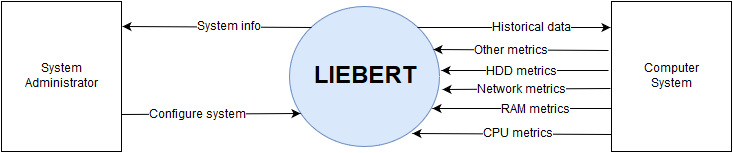
\includegraphics[width=\textwidth]{diagram-context.png}
            \caption{The context diagram}
            \label{fig:diagram-context}
        \end{figure}

        The context diagram provided in \autoref{fig:diagram-context} displays the information flow to and from the system. As said before, the autonomous nature of our system limits its reach, therefore information will only be exchanged with the computer systems that are running the application, and with potential system administrators that are either engaging in maintenance tasks or are checking on the status of the application itself. This type of diagram is also known as the \textit{Data Flow Diagram}.

    \section{Requirements}
        \subsection{Similar software}
            To better understand the requirements for system monitoring software, a survey of some of the most popular existing solutions was performed. Exploring their features and prominent characteristics allowed for a more precise specification on what shall be the focus of this project.

            \subsubsection{Nagios}
                \textit{Nagios} (\url{https://www.nagios.org/}), '\textit{the industry standard in IT infrastructure monitoring}' as it proclaims itself, is an extremely extensible monitoring solution. It doesn't come with any actual data gathering capabilities out of the box, however its plugin architecture allows users to write extensions to monitor anything from system metrics to complex applications. Nagios offers excellent alerting and early warning capabilities atop the user supplied data as well as logging, however its configuration is rather complex. It also comes with a basic but very powerful web dashboard allowing control over the software. The storage backend of \textit{Nagios} is handled by \textit{RRDtool}.
            \subsubsection{Munin}
                \textit{Munin} (\url{http://munin-monitoring.org/}) is an alerting solution similar to \textit{Nagios}, however its main focus is on ease of use. It provides near plug-and-play capabilities and simple configuration and plugin creation. \textit{Munin} uses a master - nodes architecture where
                the master node polls all child nodes for data. Plugins can be written in any language and only require that they be executable and their text output matches \textit{Munin} specifications. It also offers a simple web interface, and stores it's data using \textit{RRDtool}.
            \subsubsection{collectd}
                \textit{Collectd} (\url{https://collectd.org/}) is a minimal filtering and relaying Unix daemon with extensible architecture. Core of \textit{collectd} only provides high performance 'routing' capabilities between various input and output plugins. By default it ships with plugins for collecting cpu, network, load and memory data, as well as output plugins for CSV, RRD, and network relaying. \textit{Collectd} plugins have to be written in C and are loaded as shared modules - this makes them highly efficient and performant, however makes them incredibly difficult to make for someone who is not well-versed in C.

            \subsubsection{Feature table}
                To better understand the differences between the aforementioned monitoring solutions, a feature comparison table has been created. It shows clear difference between the features, and allows cherry-picking characteristics of each solution that should be part of \textbf{LIEBERT}.

                \begin{center}
                    \begin{tabular}{ |c|c|c|c|c| }
                        \hline
                            Features & \textbf{Nagios} & \textbf{Munin} & \textbf{collectd} & \textbf{LIEBERT}\\
                            \hline
                            \textbf{Extensible} & Yes & Yes & Yes & Extra feature\\
                            \hline
                            \textbf{Easy to extend} & No & Yes & No & Extra feature - Yes\\
                            \hline
                            \textbf{Core monitoring included} & No & Yes & Yes & Yes\\
                            \hline
                            \textbf{Web dashboard} & Yes & Yes & No & No\\
                            \hline
                            \textbf{Easy to use} & No & Yes & No & Yes\\
                            \hline
                            \textbf{Focused on performance} & No & No & Yes & Yes\\
                            \hline
                            \textbf{Cross-platform} & No & No & No & Partially\\
                        \hline
                    \end{tabular}
                \end{center}

                \paragraph{Extensibility}
                    Extensibility is not planned as an essential part of \textbf{LIEBERT}. This is due to the fact that important metric collectors will be included as part of the system core, and therefore optimized. Extensibility, if implemented will be working on the same principle as \textit{Munin}, where \textbf{LIEBERT} will call user supplied executables that will provide data in specific format recognizable by the system.

                \paragraph{Web dashboard}
                    The aim of this project is to create a highly performant system with minimal memory footprint. In order to achieve that, certain features need to be sacrificed. Web accessibility (and advanced user interaction in general) is not included in the project as such features would most probably be more resource intensive than \textbf{LIEBERT} itself.

                \paragraph{Easy to use}
                    Ease of use is probably the second most important requirement after performance. This will enable users to make use of high performance monitoring without the steep learning curve of tools such as \textit{collectd}. \textbf{LIEBERT} will strive to provide an easy setup and configuration akin to \textit{Munin}, where users should be able to get basic monitoring started just by changing a few lines in a configuration file.

                \paragraph{Performance}
                    Primary requirement of this project is performance. Features will be sacrificed to provide high performance and small memory footprint (compared to other full-featured solutions). The system will be implemented in a low level language to ensure no performance overhead arising from complex modern languages.

                \paragraph{Cross-platform}
                    Altough \textbf{LIEBERT} will not be intentionally developed for cross-platform compatibility, it will be very easy to port to other platforms due to the chosen programming language (read more in \autoref{sec:language}). In fact, most of it will be written in cross-platform compatible code and the only parts that will need rewriting are the gatherer modules which utilize native OS resources.

        \subsection{Programming language}\label{sec:language}
            In order to maximize performance of the system, care needs to be taken when choosing the language it will be implemented in. Choice of an unsuitable language might effectively 'undo' any optimizations done within the code, as the language's execution environment can be a source of large resource utilization. This is especially true for hybrid \textit{JIT} compiled languages such as Java or C\#. In the following subsections the results of surveying for potentially suitable languages can be found.

            \subsubsection{C / C++}
                \textit{C}, or "The closest you can get to assembler"\footnote{Quote from an old coworker}, is a low-level, immensly powerful and versatile language with practically zero overhead. It enables programmers to create highly optimized applications, however its 'freedom' can (and will) lead to negative side-effects such as no memory safety. \textit{C++} is an evolution of \textit{C} that added modern features on top of the old language, such as objects. These two languages would be suitable for the project, however their inherent memory unsafety can be a problem.

            \subsubsection{Go}
                \textit{Go} is a modern systems programming language created by \textit{Google}. It has seen surge of popularity since its public release in 2009, especially in recent years. It offers similar low-level system access as the \textit{C} family, however was designed for concurrent applications and therefore contains built-in concurrency and memory safety features. It also features a garbage collector found in many modern high-level languages. \textit{Go} would be a fantastic fit for \textbf{LIEBERT}, however its use of the garbage collector is a downside.

            \subsubsection{Rust}
                \textit{Mozilla}'s very own programming language \textit{Rust}, publicly announced in 2010, has seen recent surge in popularity in the same way as \textit{Go}. Rust is essentially a very low-level language akin to \textit{C}, without any additional overhead of a garbage collector that \textit{Go} has. It is also focused on concurrency and memory safety, and additionally contains so called \textit{zero-cost abstractions}. \textit{Zero-cost abstractions} are compile-time features that allow the language to have powerful features often found in higher level languages, however with practically zero overhead. This is accomplished by the \textit{Rust} compiler that performs complicated analysis and optimization, that's additionally able to perform actions such as unrolling highly complex loops \citep{asseldonk}. Notable features of the language is the lack of objects, native support for creating and distributing libraries, memory safety (mostly accomplished by the so called \textit{borrow checker}), type inference, and its focus on concurrency.

            \subsubsection{Python}
                \textit{Python} is the most popular interpreted programming language \citep{tiobe}. Years of development surprisingly allowed it to mature into a powerful and incredibly fast interpreter. It doesn't have a set goal or focus in mind, and is instead a general programming language capable of producing nearly any sort of application. \textit{Python} provides convenience features found in many high-level programming languages, such as dynamic typing or a garbage collector. Altough it is considerably fast, it's still going to suffer from overhead compared to low-level compiled programming languages.

            \subsubsection{Feature table}
                \begin{center}
                    \begin{tabular}{ |c|c|c|c|c|c| }
                        \hline
                            Features & \textbf{C / C++} & \textbf{Go} & \textbf{Rust} & \textbf{Python} & \textbf{Desired?}\\
                            \hline
                            \textbf{Low-level} & Yes & Yes & Yes & No & Yes\\
                            \hline
                            \textbf{Garbage collector} & No & Yes & No & Yes & No\\
                            \hline
                            \textbf{Dynamic typing} & No & No & No & Yes & No\\
                            \hline
                            \textbf{Conveniece features} & No & Somewhat & Yes & Yes & Yes\\
                            \hline
                            \textbf{Runtime overhead} & No & Small & No & Large & No\\
                            \hline
                            \textbf{Cross-platform} & Yes & Yes & Yes & Yes & Yes\\
                            \hline
                            \textbf{Memory safety} & No & Yes & Yes & Partially & Yes\\
                        \hline
                    \end{tabular}
                \end{center}

            \subsubsection{Conclusion}
                \paragraph{Programming language}
                    The implementation language chosen for this project is \textbf{Rust}. It features many high-level language convenience features through its \textit{zero-cost abstraction} system, focuses on concurrency, and does not come with any added overhead of the likes of a garbage collector.

                \paragraph{Development methodology}
                    Traditional methodologies such as \textit{waterfall} are becoming less and less popular in modern software development. Altough still present, they are often remnants of the old times in large corporations with established workflows. Evolving progressive teams and new companies alike are usually not in favour of such methodologies, and instead prefer modern ones such as \textit{Agile} to enable rapid feature development, leveraging continuos integration and deployment to push new releases into production as quickly as possible. This project will embrace the \textit{agile-scrum} methodology, focusing on design, development and release of features in small batches. This is relevant to the Gantt chart found in \autoref{sec:gantt}, which indicates a longer running design and development cycle in the first phase of the project that focuses on delivering a minimal working version, with short-release feature development cycles in the second phase.

        \subsection{Functional requirements}
            The system will consist of 2 applications, an \textit{Agent} and a \textit{Controller}. Each has its own set of requirements.

            \subsubsection{Agent}
                \begin{tabular}{ p{0.7cm}|p{14.5cm} }
                    \multirow{3}{*}{R1 } & \textbf{The application shall collect CPU state metrics}\\
                    \cline{2-2}
                    & The application should extract CPU load counters from the underlying operating system with as much granularity as possible. These should at least include user and system load.\\
                    \cline{2-2}
                    & Importance: \textbf{essential}
                \end{tabular}

                \vspace{0.5cm}
                \noindent
                \begin{tabular}{ p{0.7cm}|p{14.5cm} }
                    \multirow{3}{*}{R2 } & \textbf{The application shall collect RAM state metrics}\\
                    \cline{2-2}
                    & The application should extract current RAM usage from the underlying operating system. This should include utilized RAM as a minimum.\\
                    \cline{2-2}
                    & Importance: \textbf{essential}
                \end{tabular}

                \vspace{0.5cm}
                \noindent
                \begin{tabular}{ p{0.7cm}|p{14.5cm} }
                    \multirow{3}{*}{R3 } & \textbf{The application shall collect HDD state metrics}\\
                    \cline{2-2}
                    & The application should extract current disk usage from the underlying operating system. This should include the primary partition as a minimum.\\
                    \cline{2-2}
                    & Importance: \textbf{essential}
                \end{tabular}

                \vspace{0.5cm}
                \noindent
                \begin{tabular}{ p{0.7cm}|p{14.5cm} }
                    \multirow{3}{*}{R4 } & \textbf{The application shall collect network interface metrics}\\
                    \cline{2-2}
                    & The application should extract network throughput and interface information from the underlying operating system.\\
                    \cline{2-2}
                    & Importance: \textbf{essential}
                \end{tabular}

                \vspace{0.5cm}
                \noindent
                \begin{tabular}{ p{0.7cm}|p{14.5cm} }
                    \multirow{3}{*}{R5 } & \textbf{The application shall store collected data in an internal buffer}\\
                    \cline{2-2}
                    & The application should accumulate gathered metrics in an internal structure until they are ready to be sent over the network to the connected \textit{Controller} instance.\\
                    \cline{2-2}
                    & Importance: \textbf{essential}
                \end{tabular}

                \vspace{0.5cm}
                \noindent
                \begin{tabular}{ p{0.7cm}|p{14.5cm} }
                    \multirow{3}{*}{R6 } & \textbf{The application shall connect to a controller instance}\\
                    \cline{2-2}
                    & The application should establish a TCP link with a relevant controller on the network. This connection will be used to forward metric data and receive control commands.\\
                    \cline{2-2}
                    & Importance: \textbf{desired}
                \end{tabular}

                \vspace{0.5cm}
                \noindent
                \begin{tabular}{ p{0.7cm}|p{14.5cm} }
                    \multirow{3}{*}{R7 } & \textbf{The application shall forward the stored data to a connected Controller instance}\\
                    \cline{2-2}
                    & The application should periodically forward accumulated metric data to a connected \textit{Controller} instance. In case the \textit{Controller} is unavailable, it should keep accumulating data internally until the \textit{Controller} becomes available.\\
                    \cline{2-2}
                    & Importance: \textbf{desired}
                \end{tabular}

                \vspace{0.5cm}
                \noindent
                \begin{tabular}{ p{0.7cm}|p{14.5cm} }
                    \multirow{3}{*}{R8 } & \textbf{The application shall be extendable}\\
                    \cline{2-2}
                    & Users should be able to extend the gathering capabilities with custom executables providing output recognizable by the system.\\
                    \cline{2-2}
                    & Importance: \textbf{luxury}
                \end{tabular}

                \vspace{0.5cm}
                \noindent
                \begin{tabular}{ p{0.7cm}|p{14.5cm} }
                    \multirow{3}{*}{R9 } & \textbf{The user shall be able to configure all parts of the application}\\
                    \cline{2-2}
                    & The application should be configurable in all areas where it makes sense. This would include network, gathering, and storage configuration at minimum.\\
                    \cline{2-2}
                    & Importance: \textbf{desirable}
                \end{tabular}

                \vspace{0.5cm}
                \noindent
                \begin{tabular}{ p{0.7cm}|p{14.5cm} }
                    \multirow{3}{*}{R10} & \textbf{The application shall log important runtime information}\\
                    \cline{2-2}
                    & The application should print \textit{debug} / \textit{warning} / \textit{info} messages either to to \textit{stdout} or a file.\\
                    \cline{2-2}
                    & Importance: \textbf{essential}
                \end{tabular}

                \vspace{0.5cm}
                \noindent
                \begin{tabular}{ p{0.7cm}|p{14.5cm} }
                    \multirow{3}{*}{R11} & \textbf{The user shall be able to check the application's current status}\\
                    \cline{2-2}
                    & There should be a way to 'tap into' the application and review its current status. This should probably be implemented as an additional protocol over the network.\\
                    \cline{2-2}
                    & Importance: \textbf{luxury}
                \end{tabular}


            \subsubsection{Controller}
                \begin{tabular}{ p{0.7cm}|p{14.5cm} }
                    \multirow{3}{*}{R12} & \textbf{The application shall receive connections from \textit{Agents}}\\
                    \cline{2-2}
                    & The application should be able to establish TCP connections with \textit{Agents} on the network.\\
                    \cline{2-2}
                    & Importance: \textbf{essential}
                \end{tabular}

                \vspace{0.5cm}
                \noindent
                \begin{tabular}{ p{0.7cm}|p{14.5cm} }
                    \multirow{3}{*}{R13} & \textbf{The application shall authenticate connecting \textit{Agents}}\\
                    \cline{2-2}
                    & The application should implement security protocols to only allow connections from authorized \textit{Agents}.\\
                    \cline{2-2}
                    & Importance: \textbf{luxury}
                \end{tabular}

                \vspace{0.5cm}
                \noindent
                \begin{tabular}{ p{0.7cm}|p{14.5cm} }
                    \multirow{3}{*}{R14} & \textbf{The application shall receive data from connected \textit{Agents}}\\
                    \cline{2-2}
                    & The application should be able to handle historical metric data received from all connected \textit{Agents}\\
                    \cline{2-2}
                    & Importance: \textbf{essential}
                \end{tabular}

                \vspace{0.5cm}
                \noindent
                \begin{tabular}{ p{0.7cm}|p{14.5cm} }
                    \multirow{3}{*}{R15} & \textbf{The application shall store data into persistent storage}\\
                    \cline{2-2}
                    & The application should store the historical metric data received from \textit{Agents} to persistent storage (e.g. hard drive) in one of the supported formats.\\
                    \cline{2-2}
                    & Importance: \textbf{essential}
                \end{tabular}

                \vspace{0.5cm}
                \noindent
                \begin{tabular}{ p{0.7cm}|p{14.5cm} }
                    \multirow{3}{*}{R16} & \textbf{The application shall store data using plaintext format}\\
                    \cline{2-2}
                    & The application should be able to store data to persistent storage using a suitable plaintext format.\\
                    \cline{2-2}
                    & Importance: \textbf{essential}
                \end{tabular}

                \vspace{0.5cm}
                \noindent
                \begin{tabular}{ p{0.7cm}|p{14.5cm} }
                    \multirow{3}{*}{R17} & \textbf{The application shall store data using \textit{RRD} format}\\
                    \cline{2-2}
                    & The application should be able to store data to persistent storage using the format supported by \textit{RRDtool}.\\
                    \cline{2-2}
                    & Importance: \textbf{desired}
                \end{tabular}

                \vspace{0.5cm}
                \noindent
                \begin{tabular}{ p{0.7cm}|p{14.5cm} }
                    \multirow{3}{*}{R18} & \textbf{The application shall store data into a database}\\
                    \cline{2-2}
                    & The application should be able to store data into a relational database such as \textit{SQLite} or \textit{MySQL}.\\
                    \cline{2-2}
                    & Importance: \textbf{luxury}
                \end{tabular}

                \vspace{0.5cm}
                \noindent
                \begin{tabular}{ p{0.7cm}|p{14.5cm} }
                    \multirow{3}{*}{R19} & \textbf{The application shall be extendable}\\
                    \cline{2-2}
                    & The output formats of the application should be extendable using user supplied executables that accept a predefined format of the system.\\
                    \cline{2-2}
                    & Importance: \textbf{luxury}
                \end{tabular}

                \vspace{0.5cm}
                \noindent
                \begin{tabular}{ p{0.7cm}|p{14.5cm} }
                    \multirow{3}{*}{R20} & \textbf{The user shall be able to configure all parts of the application}\\
                    \cline{2-2}
                    & The application should be configurable in all areas where it makes sense. This would include network and storage configuration at minimum.\\
                    \cline{2-2}
                    & Importance: \textbf{desired}
                \end{tabular}

                \vspace{0.5cm}
                \noindent
                \begin{tabular}{ p{0.7cm}|p{14.5cm} }
                    \multirow{3}{*}{R21} & \textbf{The user shall be able to check the application's current status}\\
                    \cline{2-2}
                    & There should be a way to 'tap into' the application and review its current status. This should probably be implemented as an additional protocol over the network.\\
                    \cline{2-2}
                    & Importance: \textbf{luxury}
                \end{tabular}

                \vspace{0.5cm}
                \noindent
                \begin{tabular}{ p{0.7cm}|p{14.5cm} }
                    \multirow{3}{*}{R22} & \textbf{The user shall be able to relay commands to all connected \textit{Agents}}\\
                    \cline{2-2}
                    & The user should be able to utilize the \textit{Controller's} connections to relay commands to connected \textit{Agent} instances. This requirement is closely related to '\textit{The user shall be able to check the application's current status}'.\\
                    \cline{2-2}
                    & Importance: \textbf{luxury}
                \end{tabular}

                \vspace{0.5cm}
                \noindent
                \begin{tabular}{ p{0.7cm}|p{14.5cm} }
                    \multirow{3}{*}{R23} & \textbf{The application shall log important runtime information}\\
                    \cline{2-2}
                    & The application should print \textit{debug} / \textit{warning} / \textit{info} messages either to to \textit{stdout} or a file.\\
                    \cline{2-2}
                    & Importance: \textbf{essential}
                \end{tabular}



        \subsection{Non-functional requirements}
            \begin{tabular}{ p{0.7cm}|p{14.5cm} }
                \multirow{3}{*}{NF1} & \textbf{The system shall be built with focus on performance}\\
                \cline{2-2}
                & Maximum care should be taken when designing and developing the project to ensure maximum performance of the end result.\\
                \cline{2-2}
                & Importance: \textbf{essential}
            \end{tabular}

            \vspace{0.5cm}
            \noindent
            \begin{tabular}{ p{0.7cm}|p{14.5cm} }
                \multirow{3}{*}{NF2} & \textbf{The system shall be written in the \textit{Rust} programming language}\\
                \cline{2-2}
                & After careful consideration of multiple programming languages (discussed in \autoref{sec:language}) the \textit{Rust} programming language has been chosen due to its best feature-to-performance ratio.\\
                \cline{2-2}
                & Importance: \textbf{essential}
            \end{tabular}

            \vspace{0.5cm}
            \noindent
            \begin{tabular}{ p{0.7cm}|p{14.5cm} }
                \multirow{3}{*}{NF3} & \textbf{The system shall target the Linux operating system}\\
                \cline{2-2}
                & As discussed in \autoref{sec:scope}, primary support for Linux has been chosen due to its popularity with servers.\\
                \cline{2-2}
                & Importance: \textbf{essential}
            \end{tabular}

            \vspace{0.5cm}
            \noindent
            \begin{tabular}{ p{0.7cm}|p{14.5cm} }
                \multirow{3}{*}{NF4} & \textbf{The various system parts shall communicate through a network}\\
                \cline{2-2}
                & Due to the nature of \textit{Agent} and \textit{Controller}, network communication will be required to utilize all the features of the system.\\
                \cline{2-2}
                & Importance: \textbf{essential}
            \end{tabular}

            \vspace{0.5cm}
            \noindent
            \begin{tabular}{ p{0.7cm}|p{14.5cm} }
                \multirow{3}{*}{NF5} & \textbf{The system shall be built with focus on ease of use}\\
                \cline{2-2}
                & The system should be as easy to use as possible, ideally being able to be utilized with only a few changed lines in a configuration file.\\
                \cline{2-2}
                & Importance: \textbf{essential}
            \end{tabular}

            \vspace{0.5cm}
            \noindent
            \begin{tabular}{ p{0.7cm}|p{14.5cm} }
                \multirow{3}{*}{NF6} & \textbf{The system shall be secure}\\
                \cline{2-2}
                & The system should make use of good modern security practices to not open the network it's residing on to unauthorized entities and prevent tampering with its data.\\
                \cline{2-2}
                & Importance: \textbf{luxury}
            \end{tabular}

            \vspace{0.5cm}
            \noindent
            \begin{tabular}{ p{0.7cm}|p{14.5cm} }
                \multirow{3}{*}{NF7} & \textbf{The system shall have minimal memory footprint}\\
                \cline{2-2}
                & Due to the system's focus on performance, it should also consume minimum resource on the system it is running on.\\
                \cline{2-2}
                & Importance: \textbf{essential}
            \end{tabular}

            \vspace{0.5cm}
            \noindent
            \begin{tabular}{ p{0.7cm}|p{14.5cm} }
                \multirow{3}{*}{NF8} & \textbf{The system's data shall be accurate}\\
                \cline{2-2}
                & Maximum care should be taken to ensure the data retrieved by the system accurately represents the real state.\\
                \cline{2-2}
                & Importance: \textbf{essential}
            \end{tabular}

    \pagebreak

    \section{Use cases}
        Closed and autonomous nature of the system makes regular use case modelling rather hard, however use case modelling still remains important to uncover the various flows within an application. Therefore, instead of focusing on traditional user-oriented use cases, this section will also contain internal system flows such as metric gathering or network communication.

        \subsection{Use case diagram}
            \begin{center}
                \begin{figure}[!h]
                    \includegraphics[width=\textwidth]{diagram-usecase.png}
                    \caption{The use case diagram}
                    \label{fig:diagram-usecase}
                \end{figure}
            \end{center}

        \pagebreak

        \subsection{Use case specifications}
            \begin{longtable}{ |c|p{11.8cm}| }
                \hline
                \multicolumn{2}{|c|}{\cellcolor{lime} \textbf{UC\_1}}\\ \hline
                \cellcolor[gray]{0.9} \textbf{Use case} & Start \textit{Agent}\\ \hline
                \cellcolor[gray]{0.9} \textbf{Description} & Administrator attempts to start the \textit{Agent} application using the operating system's appropriate method\\ \hline
                \cellcolor[gray]{0.9} \textbf{Actors} & Administrator, \textit{Agent}\\ \hline
                \cellcolor[gray]{0.9} \textbf{Pre-conditions} & Application is present on target machine and target machine is running a supported platform\\ \hline
                \multicolumn{2}{|c|}{\cellcolor[gray]{0.9} \textbf{Flow of events}}\\ \hline
                \multicolumn{2}{|l|}{\cellcolor[gray]{0.9} \textbf{Normal flow}}\\ \hline
                \multicolumn{2}{|p{14cm}|}{
                    \begin{enumerate}
                        \item Administrator launches application
                        \item Application parses command line options
                        \item Application loads and parses relevant configuration file
                        \item Application attempts to connect to a configured controller
                        \item Application starts all metric gathering subsystems
                        \item Application enters normal run loop
                    \end{enumerate}
                }\\ \hline
                \multicolumn{2}{|l|}{\cellcolor[gray]{0.9} \textbf{Alternative flow}}\\ \hline
                \multicolumn{2}{|p{14cm}|}{
                    \begin{itemize}
                        \item N/A
                    \end{itemize}
                }\\ \hline
                \cellcolor[gray]{0.9} \textbf{Exceptions} &
                    \begin{itemize}
                        \item If in step 3 the application cannot find a relevant configuration file it exits with an error
                        \item If in step 3 the application cannot successfuly parse the configuration file it exits with an error
                        \item If maximum retries are exceeded in step 4 the application exits with an error
                        \item If a subsystem fails to load in step 5, the application moves it to disabled state and continues
                    \end{itemize}\\ \hline
                \cellcolor[gray]{0.9} \textbf{Post-conditions} & The application is successfuly started and running\\ \hline
            \end{longtable}

            \vspace{0.5cm}
            \noindent
            \begin{longtable}{ |c|p{11.8cm}| }
                \hline
                \multicolumn{2}{|c|}{\cellcolor{lime} \textbf{UC\_2}}\\ \hline
                \cellcolor[gray]{0.9} \textbf{Use case} & Start \textit{Controller}\\ \hline
                \cellcolor[gray]{0.9} \textbf{Description} & Administrator attempts to start the \textit{Controller} application using the operating system's appropriate method\\ \hline
                \cellcolor[gray]{0.9} \textbf{Actors} & Administrator, \textit{Controller}\\ \hline
                \cellcolor[gray]{0.9} \textbf{Pre-conditions} & Application is present on target machine and target machine is running a supported platform\\ \hline
                \multicolumn{2}{|c|}{\cellcolor[gray]{0.9} \textbf{Flow of events}}\\ \hline
                \multicolumn{2}{|l|}{\cellcolor[gray]{0.9} \textbf{Normal flow}}\\ \hline
                \multicolumn{2}{|p{14cm}|}{
                    \begin{enumerate}
                        \item Administrator launches application
                        \item Application parses command line options
                        \item Application loads and parses relevant configuration file
                        \item Application starts all configured storage subsystems
                        \item Application starts listening for \textit{Agent} connections
                        \item Application starts listening for control connections
                        \item Application enters normal run loop
                    \end{enumerate}
                }\\ \hline
                \multicolumn{2}{|l|}{\cellcolor[gray]{0.9} \textbf{Alternative flow}}\\ \hline
                \multicolumn{2}{|p{14cm}|}{
                    \begin{itemize}
                        \item N/A
                    \end{itemize}
                }\\ \hline
                \cellcolor[gray]{0.9} \textbf{Exceptions} & 
                    \begin{itemize}
                        \item If in step 3 the application cannot find a relevant configuration file it exits with an error
                        \item If in step 3 the application cannot successfuly parse the configuration file it exits with an error
                        \item If a subsystem fails to load in step 4, the application moves it to disabled state and continues; if all subsystems fail to load, the application exits with an error
                        \item If the application fails to initialize a TCP listener in step 5 or 6, it exits with an error
                    \end{itemize}\\ \hline
                \cellcolor[gray]{0.9} \textbf{Post-conditions} & The application is successfuly started and running\\ \hline
            \end{longtable}

            \vspace{0.5cm}
            \noindent
            \begin{longtable}{ |c|p{11.8cm}| }
                \hline
                \multicolumn{2}{|c|}{\cellcolor{lime} \textbf{UC\_3}}\\ \hline
                \cellcolor[gray]{0.9} \textbf{Use case} & Configure \textit{Agent}\\ \hline
                \cellcolor[gray]{0.9} \textbf{Description} & The administrator attempts to configure the \textit{Agent} application\\ \hline
                \cellcolor[gray]{0.9} \textbf{Actors} & Administrator, \textit{Agent}, \textit{Controller}\\ \hline
                \cellcolor[gray]{0.9} \textbf{Pre-conditions} & The \textit{Agent} application has been successfuly started; the \textit{Controller} application has been successfuly started and is connected to the relevant \textit{Agent} instance (for alternative flow)\\ \hline
                \multicolumn{2}{|c|}{\cellcolor[gray]{0.9} \textbf{Flow of events}}\\ \hline
                \multicolumn{2}{|l|}{\cellcolor[gray]{0.9} \textbf{Normal flow}}\\ \hline
                \multicolumn{2}{|p{14cm}|}{
                    \begin{enumerate}
                        \item Administrator opens an existing or creates a new configuration file
                        \item Administrator edits the configuration file
                        \item Administrator stops the \textit{Agent} application (if running)
                        \item Administrator starts the \textit{Agent} application - continues in \textbf{UC\_1}
                    \end{enumerate}
                }\\ \hline
                \multicolumn{2}{|l|}{\cellcolor[gray]{0.9} \textbf{Alternative flow}}\\ \hline
                \multicolumn{2}{|p{14cm}|}{
                    \begin{enumerate}
                        \item Administrator successfuly completes \textbf{UC\_5}
                        \item Administrator sends configuration command to \textit{Controller}
                        \item \textit{Controller} relays configuration command to the relevant \textit{Agent}
                        \item \textit{Agent} performs a run-time reconfiguration based on the command received
                    \end{enumerate}
                }\\ \hline
                \cellcolor[gray]{0.9} \textbf{Exceptions} & 
                    \begin{itemize}
                        \item If the command received by \textit{Agent} in \textit{Alternative flow step 3} is invalid, it is discarded and a warning is emitted 
                    \end{itemize}\\ \hline
                \cellcolor[gray]{0.9} \textbf{Post-conditions} & The \textit{Agent} application is successfuly running with the new configuration\\ \hline
            \end{longtable}

            \vspace{0.5cm}
            \noindent
            \begin{longtable}{ |c|p{11.8cm}| }
                \hline
                \multicolumn{2}{|c|}{\cellcolor{lime} \textbf{UC\_4}}\\ \hline
                \cellcolor[gray]{0.9} \textbf{Use case} & Configure \textit{Controller}\\ \hline
                \cellcolor[gray]{0.9} \textbf{Description} & The administrator attempts to configure the \textit{Controller} application\\ \hline
                \cellcolor[gray]{0.9} \textbf{Actors} & Administrator, \textit{Controller}\\ \hline
                \cellcolor[gray]{0.9} \textbf{Pre-conditions} & The \textit{Controller} application has been successfuly started\\ \hline
                \multicolumn{2}{|c|}{\cellcolor[gray]{0.9} \textbf{Flow of events}}\\ \hline
                \multicolumn{2}{|l|}{\cellcolor[gray]{0.9} \textbf{Normal flow}}\\ \hline
                \multicolumn{2}{|p{14cm}|}{
                    \begin{enumerate}
                        \item Administrator opens an existing or creates a new configuration file
                        \item Administrator edits the configuration file
                        \item Administrator stops the \textit{Controller} application (if running)
                        \item Administrator starts the \textit{Controller} application - continues in \textbf{UC\_2}
                    \end{enumerate}
                }\\ \hline
                \multicolumn{2}{|l|}{\cellcolor[gray]{0.9} \textbf{Alternative flow}}\\ \hline
                \multicolumn{2}{|p{14cm}|}{
                    \begin{enumerate}
                        \item Administrator successfuly completes \textbf{UC\_5}
                        \item Administrator sends configuration command to \textit{Controller}
                        \item \textit{Controller} performs run-time reconfiguration based on the command received
                    \end{enumerate}
                }\\ \hline
                \cellcolor[gray]{0.9} \textbf{Exceptions} & 
                    \begin{itemize}
                        \item If the command received by the \textit{Controller} in \textit{Alternative flow step 2} is invalid, it is discarded and a warning is emitted
                    \end{itemize}\\ \hline
                \cellcolor[gray]{0.9} \textbf{Post-conditions} & The \textit{Controller} application is successfuly running with the new configuration\\ \hline
            \end{longtable}

            \vspace{0.5cm}
            \noindent
            \begin{longtable}{ |c|p{11.8cm}| }
                \hline
                \multicolumn{2}{|c|}{\cellcolor{lime} \textbf{UC\_5}}\\ \hline
                \cellcolor[gray]{0.9} \textbf{Use case} & Send commands\\ \hline
                \cellcolor[gray]{0.9} \textbf{Description} & Administrator attempts to control the running \textit{Controller} or \textit{Agent} instances\\ \hline
                \cellcolor[gray]{0.9} \textbf{Actors} & Administrator, \textit{Controller}, \textit{Agent}\\ \hline
                \cellcolor[gray]{0.9} \textbf{Pre-conditions} & Administrator has correct version of the \textbf{LIEBERT} CLI tool; \textit{Controller} has been successfuly started; \textit{Agent} has been successfuly started (for alternative flow)\\ \hline
                \multicolumn{2}{|c|}{\cellcolor[gray]{0.9} \textbf{Flow of events}}\\ \hline
                \multicolumn{2}{|l|}{\cellcolor[gray]{0.9} \textbf{Normal flow}}\\ \hline
                \multicolumn{2}{|p{14cm}|}{
                    \begin{enumerate}
                        \item Administrator opens the \textbf{LIEBERT} CLI application and establishes a connection with a \textit{Controller}
                        \item Administrator sends commands to controller using the CLI application
                    \end{enumerate}
                }\\ \hline
                \multicolumn{2}{|l|}{\cellcolor[gray]{0.9} \textbf{Alternative flow}}\\ \hline
                \multicolumn{2}{|p{14cm}|}{
                    \begin{enumerate}
                        \item Administrator opens the \textbf{LIEBERT} CLI application and establishes a connection with a \textit{Controller}
                        \item Administrator sends a command telling the \textit{Controller} to switch to \textit{Agent} control model
                        \item Administrator sends commands to controller which get relayed to the relevant \textit{Agent} instance
                    \end{enumerate}
                }\\ \hline
                \cellcolor[gray]{0.9} \textbf{Exceptions} & 
                    \begin{itemize}
                        \item If the connection fails in \textit{Normal flow step 1} or \textit{Alternative flow step 1}, the CLI tool exits with an error
                        \item If the \textit{Agent} selected in \textit{Alternative flow step 2} is invalid, \textit{Controller} responds with an error
                        \item If the command sent in \textit{Normal flow step 2} or \textit{Alternative flow step 3} is invalid, it is discarded by the receiving node
                    \end{itemize}\\ \hline
                \cellcolor[gray]{0.9} \textbf{Post-conditions} & Administrator has established a connection with a \textit{Controller} using the CLI tool and is able to send commands\\ \hline
            \end{longtable}

            \vspace{0.5cm}
            \noindent
            \begin{longtable}{ |c|p{11.8cm}| }
                \hline
                \multicolumn{2}{|c|}{\cellcolor{lime} \textbf{UC\_6}}\\ \hline
                \cellcolor[gray]{0.9} \textbf{Use case} & Check status\\ \hline
                \cellcolor[gray]{0.9} \textbf{Description} & Administrator attempts to check the status of a specific \textit{Agent} or \textit{Controller} instance\\ \hline
                \cellcolor[gray]{0.9} \textbf{Actors} & Administrator, \textit{Controller}, \textit{Agent}\\ \hline
                \cellcolor[gray]{0.9} \textbf{Pre-conditions} & Relevant \textit{Controller} and \textit{Agent} instances have been successfuly started and are running\\ \hline
                \multicolumn{2}{|c|}{\cellcolor[gray]{0.9} \textbf{Flow of events}}\\ \hline
                \multicolumn{2}{|l|}{\cellcolor[gray]{0.9} \textbf{Normal flow}}\\ \hline
                \multicolumn{2}{|p{14cm}|}{
                    \begin{enumerate}
                        \item Administrator successfuly completes \textbf{UC\_5}
                        \item Administrator sends a check status command
                        \item \textit{Controller} relays the command to the specified node
                        \item \textit{Controller} responds with the response received from the specified node
                    \end{enumerate}
                }\\ \hline
                \multicolumn{2}{|l|}{\cellcolor[gray]{0.9} \textbf{Alternative flow}}\\ \hline
                \multicolumn{2}{|p{14cm}|}{
                    \begin{itemize}
                        \item N/A
                    \end{itemize}
                }\\ \hline
                \cellcolor[gray]{0.9} \textbf{Exceptions} & 
                    \begin{itemize}
                        \item If the node requested in step 2 is invalid, \textit{Controller} responds with an error
                    \end{itemize}\\ \hline
                \cellcolor[gray]{0.9} \textbf{Post-conditions} & Administrator is presented with status of the relevant node\\ \hline
            \end{longtable}

            \vspace{0.5cm}
            \noindent
            \begin{longtable}{ |c|p{11.8cm}| }
                \hline
                \multicolumn{2}{|c|}{\cellcolor{lime} \textbf{UC\_7}}\\ \hline
                \cellcolor[gray]{0.9} \textbf{Use case} & Transmit gathered metrics\\ \hline
                \cellcolor[gray]{0.9} \textbf{Description} & \textit{Agent} attempts to transmit metric data held in its internal buffer to a connected \textit{Controller} instance\\ \hline
                \cellcolor[gray]{0.9} \textbf{Actors} & \textit{Agent}, \textit{Controller}\\ \hline
                \cellcolor[gray]{0.9} \textbf{Pre-conditions} & The relevant \textit{Agent} and \textit{Controller} isntances have been successfuly started\\ \hline
                \multicolumn{2}{|c|}{\cellcolor[gray]{0.9} \textbf{Flow of events}}\\ \hline
                \multicolumn{2}{|l|}{\cellcolor[gray]{0.9} \textbf{Normal flow}}\\ \hline
                \multicolumn{2}{|p{14cm}|}{
                    \begin{enumerate}
                        \item \textit{Agent} retrieves momentary metric data from its internal buffer
                        \item \textit{Agent} removes the retrieved data from the internal buffer
                        \item \textit{Agent} encodes the retrieved data into a format suitable for network transmission
                        \item \textit{Agent} sends the encoded data to the connected \textit{Controller} instance
                        \item \textit{Agent} starts again from step 1 if the internal buffer is not empty
                    \end{enumerate}
                }\\ \hline
                \multicolumn{2}{|l|}{\cellcolor[gray]{0.9} \textbf{Alternative flow}}\\ \hline
                \multicolumn{2}{|p{14cm}|}{
                    \begin{itemize}
                        \item N/A
                    \end{itemize}
                }\\ \hline
                \cellcolor[gray]{0.9} \textbf{Exceptions} & 
                    \begin{itemize}
                        \item If there is no data in the internat buffer in step 1, \textit{Agent} halts this task until the internal buffer is supplied with data
                        \item If the transmission in step 3 fails, \textit{Agent} stores the retrieved data back into the internal buffer and emits a warning
                    \end{itemize}\\ \hline
                \cellcolor[gray]{0.9} \textbf{Post-conditions} & X\\ \hline
            \end{longtable}

            \vspace{0.5cm}
            \noindent
            \begin{longtable}{ |c|p{11.8cm}| }
                \hline
                \multicolumn{2}{|c|}{\cellcolor{lime} \textbf{UC\_8}}\\ \hline
                \cellcolor[gray]{0.9} \textbf{Use case} & Gather metrics\\ \hline
                \cellcolor[gray]{0.9} \textbf{Description} & The \textit{Agent} application attempts to gather metric data using one of its gathering subsystems\\ \hline
                \cellcolor[gray]{0.9} \textbf{Actors} & \textit{Agent}, Operating System, \textit{Controller}\\ \hline
                \cellcolor[gray]{0.9} \textbf{Pre-conditions} & The \textit{Agent} application has been successfuly started; the \textit{Controller} application has been successfuly started and link with \textit{Agent} established (for alternative flow 2)\\ \hline
                \multicolumn{2}{|c|}{\cellcolor[gray]{0.9} \textbf{Flow of events}}\\ \hline
                \multicolumn{2}{|l|}{\cellcolor[gray]{0.9} \textbf{Normal flow}}\\ \hline
                \multicolumn{2}{|p{14cm}|}{
                    \begin{enumerate}
                        \item The application invokes one of its core gathering subsystems
                        \item Gathering subsystems requests metric data from the underlying operating system
                        \item Gathering subsystem transforms data into format understood by the \textit{Agent}
                        \item \textit{Agent} stores the data into its internal buffer
                    \end{enumerate}
                }\\ \hline
                \multicolumn{2}{|l|}{\cellcolor[gray]{0.9} \textbf{Alternative flow}}\\ \hline
                \multicolumn{2}{|p{14cm}|}{
                    \begin{enumerate}
                        \item The application invokes a plugin gathering subsystem
                        \item Subsystem calls a user supplied executable and parses the output
                        \item Subsystem transforms the data and hands it to the \textit{Agent}
                        \item \textit{Agent} stores the data in its internal buffer
                    \end{enumerate}
                }\\ \hline
                \multicolumn{2}{|l|}{\cellcolor[gray]{0.9} \textbf{Alternative flow 2}}\\ \hline
                \multicolumn{2}{|p{14cm}|}{
                    \begin{enumerate}
                        \item A user has requested a run of a specific gathering subsystem using a remote command
                        \item \textit{Agent} invokes the requested gathering subsystem
                        \item Gathering subsystem retrieves, transforms and hands data back to the \textit{Agent}
                        \item \textit{Agent} sends retrieved data back to the requesting administrator
                    \end{enumerate}
                }\\ \hline
                \cellcolor[gray]{0.9} \textbf{Exceptions} & 
                    \begin{itemize}
                        \item If a gathering subsystem fails to transform the retrieved data (\textit{Normal flow step 3}, \textit{Alternative flow step 3}, \textit{Alternative flow 2 step 3}), it hands the \textit{Agent} an error message; \textit{Agent} emits a warning and stores a value indicating an error
                        \item If the executable in \textit{Alternative flow step 2} cannot be executed, the specific plugin subsystem is moved to disabled state and a warning is emitted
                        \item If \textit{Agent} cannot hold any more data in its internal buffer due to memory limits, the \textit{Agent} application exits with an error
                    \end{itemize}\\ \hline
                \cellcolor[gray]{0.9} \textbf{Post-conditions} & The \textit{Agent} application expanded its internal buffer with newly collected metric data; the administrator is presented with the requested metric data (alternative flow 2)\\ \hline
            \end{longtable}

            \vspace{0.5cm}
            \noindent
            \begin{longtable}{ |c|p{11.8cm}| }
                \hline
                \multicolumn{2}{|c|}{\cellcolor{lime} \textbf{UC\_9}}\\ \hline
                \cellcolor[gray]{0.9} \textbf{Use case} & Save data\\ \hline
                \cellcolor[gray]{0.9} \textbf{Description} & The \textit{Controller} attempts to save data into persistent storage\\ \hline
                \cellcolor[gray]{0.9} \textbf{Actors} & \textit{Controller}, Filesystem\\ \hline
                \cellcolor[gray]{0.9} \textbf{Pre-conditions} & The \textit{Controller} application and at least a single connected \textit{Agent} application have been successfuly started\\ \hline
                \multicolumn{2}{|c|}{\cellcolor[gray]{0.9} \textbf{Flow of events}}\\ \hline
                \multicolumn{2}{|l|}{\cellcolor[gray]{0.9} \textbf{Normal flow}}\\ \hline
                \multicolumn{2}{|p{14cm}|}{
                    \begin{enumerate}
                        \item \textit{Controller} receives metric data from a connected \textit{Agent} instance
                        \item \textit{Controller} invokes a configured storage subsystem to store the new data
                        \item Storage subsystem stores the data into persistent storage
                        \item Repeat from step 2 for each configured storage subsystem
                    \end{enumerate}
                }\\ \hline
                \multicolumn{2}{|l|}{\cellcolor[gray]{0.9} \textbf{Alternative flow}}\\ \hline
                \multicolumn{2}{|p{14cm}|}{
                    \begin{itemize}
                        \item N/A
                    \end{itemize}
                }\\ \hline
                \cellcolor[gray]{0.9} \textbf{Exceptions} & 
                    \begin{itemize}
                        \item If the metric data received in step 1 is in invalid format it is discarded and a warning is emitted
                        \item If an invoked storage subsystem experiences a failure in step 3 it is moved to disabled state and a warning is emitted
                        \item If there are no enabled storage subsystems the application exits with an error
                    \end{itemize}\\ \hline
                \cellcolor[gray]{0.9} \textbf{Post-conditions} & Metric data retrieved from a connected \textit{Agent} instance is saved to persistent storage\\ \hline
            \end{longtable}

            

    \section{Domain model}
        \textit{Rust}, the chosen programming language (read more in \autoref{sec:language}), is not object-oriented. Therefore, a standard class diagram-based domain model cannot be created. \textit{Rust} still supports the notion of variable and function protection, however it implements these features with a file-scope, instead of a class-scope, approach. Due to this the domain model found in \autoref{fig:diagram-class} will mostly represent entities grouped together in files instead of classes.

        \subsection{Diagram}
            \begin{center}
                \begin{figure}[!h]
                    \includegraphics[width=\textwidth]{diagram-class.png}
                    \caption{The domain model}
                    \label{fig:diagram-class}
                \end{figure}
            \end{center}



    \begin{landscape}
    \section{Appendix A - Gantt chart}\label{sec:gantt}
        \begin{figure}[!htb]
            \begin{ganttchart}[
                vgrid,
                hgrid,
                x unit=1.2cm,
                link/.style={-latex, draw=red, fill=red}
            ]{1}{16}
                \gantttitle{September}{2}
                \gantttitle{October}{2}
                \gantttitle{November}{2}
                \gantttitle{December}{2}
                \gantttitle{January}{2}
                \gantttitle{February}{2}
                \gantttitle{March}{2}
                \gantttitle{April}{2} \\

                \ganttbar{Requirements}{1}{6}
                \ganttbar[inline]{further requirement discovery}{8}{16} \\
                \ganttbar{Architecture}{4}{8} \\
                \ganttbar{Protocols}{4}{10} \\
                \ganttbar{Rust basics}{1}{6} \\
                \ganttbar{Initial version}{4}{9} \\
                \ganttbar{Features}{10}{16}
                \ganttbar[inline]{agile - scrum}{10}{16}\\
                \ganttbar{Report}{3}{6}
                \ganttbar[inline]{Requirements}{3}{6}
                \ganttbar[inline]{Final report}{10}{16}

                \ganttlink[link type=f-s]{elem5}{elem6}
                \ganttlink{elem0}{elem1}
                \ganttlink{elem9}{elem10}
            \end{ganttchart}
            \caption{Gantt chart from the initial \textit{project proposal}}
            \label{fig:diagram-gantt}
        \end{figure}
    \end{landscape}

    \bibliographystyle{agsm}
    \bibliography{requirements}

\end{document}
    \clearpage
    \section{Design}
    This chapter documents the design of the application, as well as the reasoning behind choices that were made. It tries to enable the reader to understand the architecture of the application regardless of any implementation details, and does not assume the reader has any knowledge of the implementation specifics, nor the underlying platform.
    
    \subsection{Server - client architecture}\label{sec:architecture}
        \textsc{Liebert} consists of two separate applications, the so-called \textit{Agent} (client) and a \textit{Controller} (server). This solution has been chosen both because it is de facto an industry standard (see \textit{Munin}, \textit{Nagios}), and because it simply makes sense. A different approach could entail having a single client application that would perform collection and storage tasks at the same time, this however is less than ideal, as it would violate the core concept of this project - minimal resource usage on the client side, as well as increase the burden on the storage backend (e.g. database), with potentially thousands of clients keeping connections open indefinitely.
        
        A client - server architecture brings numerous benefits over the aforementioned approach. It allows processing  to be done on the received data, possibly performing custom normalization or filtering logic. From an infrastructure angle, it enables the creation of a load-balancer, a server-like application that the clients would connect to; however instead of persisting the data into storage, it would perform buffering instead, and send data to the real server periodically, potentially with utilizing compression. Such load-balancers could be placed between network segments in large networks, where hundreds, or thousands, of machines constantly transferring data to a centralized location would create network congestion.
        
        \subsubsection{Agent}
            \textit{Agents} are the applications residing on each individual monitored endpoint. The program should be distributed and installed on all systems where monitoring is desired. \textit{Agents} gather system metrics specified in the configuration, connect to a \textit{Controller} instance, and transmit gathered metrics to it. In the event of loss of connection, \textit{Agent} should buffer data and periodically attempt to re-establish a \textit{Controller} connection.
            
        \subsubsection{Controller}
            Application called the \textit{Controller} is the central part of the platform. It should reside on a single computer system and accept connections from \textit{Agents} on the network. After receiving data from a connected \textit{Agent}, it should transfer it into persistent storage based on the configuration. In the future a \textit{Controller} could potentially be used to issue run-time commands to connected \textit{Agents}, allowing reconfiguration or status checks.
            
    \subsection{Network protocol}
        As \textsc{Liebert} is built using the client-server architecture (see \autoref{sec:architecture}), it is imperative that network communication will be involved. This implies that a suitable protocol must be chosen or developed. Originally there was hope that a tailor-made protocol could be developed using a tool such as  \textit{protobuf}\footnote{Networking library widely popular for protocol implementation in C++ and other languages}, however no such library was available for the chosen implementation language (\textit{Rust}). Manual protocol implementation would be out of scope of this project, potentially complex enough for its own project, therefore it has been decided that all network communication would be done using a simple string protocol.
        
        The network protocol specification can be found in \textbf{Appendix A} (\autoref{apd:network}).
        
    \clearpage
    \section{Implementation}
    In the following chapter the implementation details of the application will be described. It covers most of the application code and the design decisions around it, as well as some more theoretical content relating to the chosen implementation language \textit{Rust}. It finishes off with a closer look at some of the notable issues that arose during development, as well as various accomplishments that the reader would not have otherwise thought about.

    \subsection{Rust}
        The chosen implementation language for the project is \textit{Rust}, more details on the decision-making surrounding this choice can be found in \autoref{sec:language}.
        
        Rust is a very low-level programming language, similar in style and functionality to C, however it is built with a "memory safety first" approach. What this means in practice is that the compiler's static analysis detects most, if not all, ways of unsafe memory access and manipulation patterns, and fails the compilation if such a mistake is detected. It is possible to override these checks by using \textit{unsafe} code blocks, this is however mostly only used in \textit{FFI}\footnote{Foreign Function Interface - used for interaction with libraries written in other languages}, as idiomatic \textit{Rust} can, and should, be written with fully memory-safe code.
        
        The advanced static analysis of the compiler is known as \textit{zero-cost abstractions}. This name is derived from the fact that most of the features of \textit{Rust} come at absolutely zero overhead, because they are bound to the compilation phase - generally, if there is a problem with the code, it will fail to compile. This is in stark contrast with most other programming languages, which often encounter possibly hard to debug run-time errors. With \textit{Rust}, encountering a run-time error is very rare if the code is idiomatic. It is still possible for the program to crash, this is however usually caused either by a system error (e.g. out of memory), or by a \textit{thread panic} - a crash manually called by the programmer, or automatically generated if a failure case is left unhandled (which is once again a conscious choice of the programmer). In addition to memory safety, \textit{Rust} contains other convenience features which, once again, usually come with zero or minimal overhead. One of these are what other languages call \textit{optional types}. In \textit{Rust}, there are two kinds of \textit{optional types}: an \textit{Option} and a \textit{Result}. These can either depict a result of an operation that returns \textit{something} or \textit{nothing}, or a choice between \textit{something} and an \textit{error}. Considering the language doesn't have exceptions, these \textit{optional types} make it a breeze when an operation should return a value, however also has a chance of failure. The \textit{Option} type is a special kind of \textit{Result} that doesn't return an \textit{error} but a \textit{nothing} - this becomes very useful when an operation doesn't have to return a value; normally it would have to allocate an empty structure to return (e.g. array or hashmap), with the \textit{Option} type it can return a more simple \textit{nothing} value.
        
        The learning curve of the language isn't very steep, unless one wants to delve into advanced topics. If there's familiarity with a strongly-typed programming language such as C\# or Java, covering the basics of \textit{Rust} will take minimal time (even less if one is familiar with low level languages such as C or C++). The hardest part about learning the language is probably trying to write idiomatic code, as it will require forgetting standard practices from other languages for which \textit{Rust} provides a better, more idiomatic way (e.g. correct usage of the \textit{optional types}).
        
        I have personally started learning \textit{Rust} about half a year before fully starting the development of the project. The reasoning behind such an early start was that I would like to acquire at least semi-intermediate knowledge of the language and its best practices before using it for such a large project as this one. The most helpful resources were the "official \textit{Rust} book" \cite{rust-book}, and because I'm a large fan of reading actual documentation (which seems to be rare these days\footnote{Personal opinion formed by observation of my peers}) I also enjoyed the official library reference. In addition to these resources I read countless articles, blog posts, and other forms of online communications while either trying to solve a problem, or just while generally catching up with the news (\textit{Rust} is very popular on numerous online forums related to programming or technology).
        
    \subsection{Threading model}\label{sec:threads}
        \textsc{Liebert} utilizes a fairly complex threading model. This comes from the fact that currently there is no asynchronous I/O in \textit{Rust}. As most functions of the application are I/O-bound, be it network or the local filesystem, they require a separate thread to be spawned as to not impede the functionality of the rest of the application.
        
        Due to memory safety and parallelism being a cornerstone of \textit{Rust}, creation and management of threads is extremely simple. This meant that the usage of threads extended beyond I/O bound tasks, and is used to divide the application into independently running "modules". Utilizing this approach also means that data can be easily processed or reformatted when being exchanged between different "modules" (read more in \autoref{sec:data-flow}). An introspection into \textsc{Liebert}'s threads as seen by the Linux utility \textit{htop} can be seen in \autoref{fig:thread-list}. Note that each thread is also appropriately named, so that they can be easily analyzed.
    
            \begin{figure}[!htb]
                \centering
                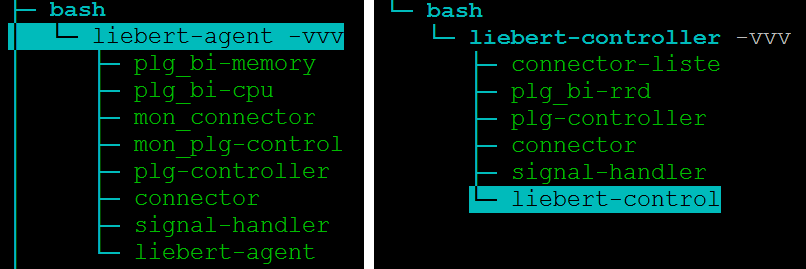
\includegraphics[width=\textwidth]{liebert-threads.png}
                \caption{\textsc{Liebert}'s thread list in \textit{htop}}
                \label{fig:thread-list}
            \end{figure}
        
        \subsubsection{Watchdog}
            With many running threads comes the issue of synchronization and thread management. To assist in this, a \textit{Watchdog} utility has been developed that is used for thread monitoring and synchronization. Currently, it's most important use case is to synchronize threads on application exit. When the user initiates a shutdown, a \textit{shutdown message} (read more in \autoref{sec:message-queue}) is sent to important threads that potentially need to do finalization before exiting. After the shutdown messages are sent, \textit{Watchdog} is used to wait for these threads to quit (handling all error scenarios gracefully), and the application exits, killing all non-important threads immediately.
        
        \subsubsection{Drawbacks}
            Unfortunately, this method has brought in some unforeseen drawbacks. Even though maximum care has been taken during development to reduce memory usage to a minimum, utilizing the multi-thread model has rendered most of these efforts rather meaningless. This is caused by the operating system allocating separate stack space for each thread. The specific initial size of this allocation varies across operating systems, and as such the application's memory consumption cannot be safely predicted. On Linux, \textit{Rust} provides an undocumented way of modifying the initial stack size as seen in  \autoref{fig:code-stack-memory-set}.
            
            \begin{figure}[!htb]
                \centering
                \begin{BVerbatim}
devel:~$ RUST_MIN_STACK=49000 ./target/release/liebert-controller
                \end{BVerbatim}
                \caption{Adjusting initial stack size by using an environment variable}
                \label{fig:code-stack-memory-set}
            \end{figure}
            
            This however seems to have some sort of a lower limit, as even though the lowest we managed to get using this approach was \textbf{4.9kB} (the option appears to be in bytes; lower values started throwing segmentation faults during application initialization), the resulting threads always allocated a minimum of \textbf{2MB}. We can look up detailed memory consumption information using the \textit{pmap} utility, invoked with the \textit{-x} flag for extended details.
            
            \begin{figure}[!htb]
                \centering
                \begin{BVerbatim}
devel:~$ ./target/release/liebert-controller
devel:~$ pmap -x <pid> | sort -nk 2 | tail -n 5
00007f6b161be000    2048       0       0 ----- libc-2.21.so
00007f6b13a00000    4096      48      48 rw---   [ anon ]
00007f6b14c00000    4096      24      24 rw---   [ anon ]
00007f6b15600000    6144     344     344 rw---   [ anon ]
00007f6b14200000    8192     116     116 rw---   [ anon ]
                \end{BVerbatim}
                \caption{Controller memory footprint using stock stack size}
                \label{fig:code-stack-memory-stock}
            \end{figure}
            
            Inspecting \autoref{fig:code-stack-memory-stock}, we see that our threads utilize \textbf{8MB}, \textbf{6MB}, \textbf{4MB} and \textbf{2MB} (not included in the figure). The largest thread is most probably the main thread, as \textit{Rust} usually allocates \textbf{8MB} for this thread on Linux, and it cannot be brought lower using the \textit{RUST\_MIN\_STACK} environment variable. The cause of the size of the rest of the threads is unknown, as they seem to randomly vary between 2, 4, and 6 megabytes. Note that you can find the full output of the \textit{pmap} utility for the default settings of \textit{liebert-controller} in \textbf{Appendix B} (\autoref{apd:pmap-controller}), and \textit{liebert-agent} in \textbf{Appendix C} (\autoref{apd:pmap-agent}).
            
            Trying to get more insight into the thread memory usage and relevance of the mysterious environment variable, we can try running the application with an exorbitant minimum stack size to determine if the environment variable in fact does something or not (\autoref{fig:code-stack-memory-custom}).
            
            \begin{figure}[!htb]
                \centering
                \begin{BVerbatim}
devel:~$ RUST_MIN_STACK=12000000 ./target/release/liebert-controller
devel:~$ pmap -x <pid> | sort -nk 2 | tail -n 5
00007fb852fab000   11716      12      12 rw---   [ anon ]
00007fb853b1d000   11716      12      12 rw---   [ anon ]
00007fb85208f000   13764      28      28 rw---   [ anon ]
00007fb85468f000   15812     348     348 rw---   [ anon ]
00007fb850e8f000   17860     116     116 rw---   [ anon ]
                \end{BVerbatim}
                \caption{Controller memory footprint using custom stack size}
                \label{fig:code-stack-memory-custom}
            \end{figure}
            
            We can see a curious phenomenon happening in \autoref{fig:code-stack-memory-custom}. Even though the stock 8MB was more than enough for the main thread, once we set the minimum stack size to 12MB, it ended up allocating more than \textbf{17MB}. The reason for this is unknown, and a closer look on the inner working of threads in \textit{Rust} (or in general) would be required, however is out of scope of this project. The same situation occurs with some of the other threads as well, as we can see that previously they consumed 6MB or less, now they take up up to almost \textbf{16MB}. We can probably assume that the threads that allocated ~12MB are the same ones that previously allocated 2MB (no thread ever allocated less regardless of the stack size setting).

            
    
    \subsection{Data flow}\label{sec:data-flow}
        The modular nature of the application allows for a quite peculiar data flow. This is a direct consequence of the multi-threading model described in the previous section, as the data needs to be moved safely and efficiently between different threads. This is done using a \textit{message queue} (read more in the next section). The application contains the following data-related modules:
        
        \textbf{Core} - Application's main event loop. Data passing from one end of the application uses it to get routed to the other end. Additionally used for system events such as initiating a shutdown.
        
        \textbf{Connector} - Used for connecting to a controller and receiving commands (\textit{Agent}), or for spawning read / write threads for incoming connections (\textit{Controller})).
        
        \textbf{Plugin Controller} - Handles available gatherer or storage backends. Forwards data received from \textbf{Core} to appropriate storage backends (\textit{Controller}.
        
        \textbf{Signal Handler} - Special purpose thread monitoring interrupt signals. Sends a \textit{shutdown message} to \textbf{Core} if an interrupt signal is detected (\textit{SIGINT} or \textit{SIGTERM}).
        
        \textbf{Plugin Threads} - Individual threads running gatherer or storage backends. Send gathered data directly to \textbf{Core} (\textit{Agent}), or receive data from a \textbf{Plugin Controller} (\textit{Controller)}.
        
        \textbf{Connection Threads} - Threads spawned for communicating with connected \textit{Agents}.
    
        \begin{figure}[!htb]
            \centering
            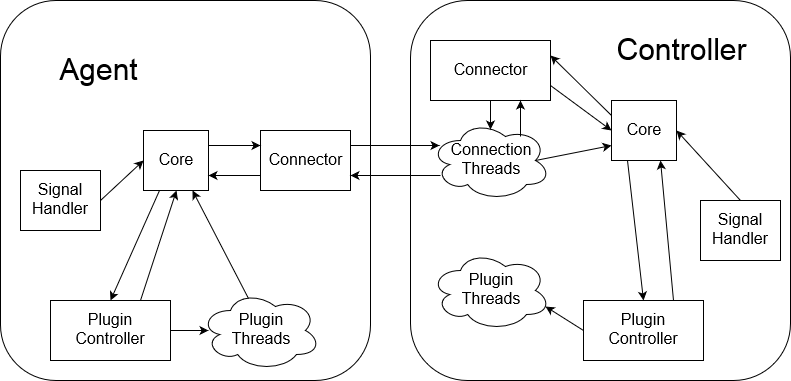
\includegraphics[width=\textwidth]{diagram-dataflow.png}
            \caption{Data flow within both applications}
            \label{fig:diagram-dataflow}
        \end{figure}
    
    \subsection{Message queue}\label{sec:message-queue}
        Due to the heavy threading within both applications, a safe and efficient way of passing data between threads had to be used. This is accomplished by using the \textit{Rust} primitive known as \textbf{channels}. These provide a memory-safe way of exchanging data between threads. Creating a channel results in two items: a \textit{sender} and a \textit{receiver}. By using \textit{Rust's} memory safety traits, channels are always restricted to a single \textit{receiver} and an unlimited number of \textit{senders}. The \textit{senders} provide a quasi-atomic means of enqueueing any sort of structure or value that can later be sequentially read through the relevant \textit{receiver}. The \textsc{Liebert} standardized structure for exchanging data between threads is a \textit{Message}, which can be seen in \autoref{fig:code-message-agent}. Note that the specific message implementation varies slightly between the two applications due to optimization reasons (more details about this are in \autoref{sec:shared-code}).
    
    \subsection{Built-in collectors}
        As stated in the requirements, the application must come with a set of built-in metric gatherers. This is a cornerstone of the project because the application only guarantees maximum performance with the built-in gatherers, as opposed to external plugins. The version of the application at the time of writing this report only contains the essential gatherers: CPU and memory.
    
        \subsubsection{CPU}
            There are multiple ways of retrieving CPU statistics under Linux. Many of them have been considered before implementation of this module, including \textit{mpstat}, \textit{/proc/stat}, \textit{top} or the average load data in \textit{uptime}. Due to the high-performance nature of this project, an approach using \textit{/proc/stat} has been chosen. Most, if not all, of the other choices required spawning an external process which incurs an unpredictable performance and memory overhead, as well as no guarantee of accurate results. The final solution reads raw CPU stats, or so called \textit{jiffies} \footnote{Jiffies are the amount of time a CPU spent on a task, they typically represent hundredths of a second}, from the system's \textit{/proc/stat} file and calculates the CPU usage accordingly. This, apart from being fast, has the added benefit of being able to calculate the exact CPU usage between any two moments in time.
        
        \subsubsection{Memory}
            The memory gatherer utilizes the standard and simple \textit{/proc/mem} file which provides detailed break-down of current memory state. More specifically, it extracts the \textbf{total}, \textbf{free}, \textbf{buffers}, and \textbf{cache} fields. These are the most important and well-known memory metrics and can be used to gain valuable insight into the current state of the system's memory.
        
    \subsection{Configurability}\label{sec:config}
        As per the original requirement, \textsc{Liebert} has been written with configurability in mind. Many parts of the application have ties to the in-memory configuration already, often even for settings that aren't available to be configured (yet). The in-memory configuration is built at the application's initialization inception, in fact it is only preceded by the creation of the main event loop send / receive channel. The configuration construction consists of two distinct but both very important steps.
        
        First, a configuration structure gets created from the command line arguments passed to the application. This is accomplished by using the handy \textbf{clap} library, which immensly eases the creation and management of command line arguments. The arguments get processed by \textbf{clap}, and get transferred into a generic configuration key-value structure. At the time of writing this report, only the \textit{-v} and \textit{-c} flags are available. These are used to specify the desired logging verbosity level, and the location of the relevant configuration file. They are both so-called \textit{global} configuration options, as they are included in both applications using shared code. Note that applications don't currently have any individual command line options, however the infrastructure for them is ready. All that needs to be done is specify the options and they will automatically work in the same way as the currently available \textit{global} ones. It is also worth mentioning that the options default to a sensible preset value if they are omitted from the command line, therefore both applications can be safely run without either the \textit{-c} or \textit{-v} flag. An automatically generated help menu is available by using the \textit{-h} or \textit{--help} switch, an example can be seen in \autoref{fig:agent-help}.
        
        \begin{figure}[!htb]
            \centering
            \begin{BVerbatim}
Liebert Agent 0.2.0
(c) Martin Kukura
Endpoint application of the Liebert monitoring platform.

USAGE:
liebert-agent [FLAGS] [OPTIONS]
FLAGS:
-h, --help       Prints help information
-V, --version    Prints version information
-v, --verbose    Verbose output
OPTIONS:
-c, --conf <conf>    Path to the configuration file
            \end{BVerbatim}
            \caption{Help output printed by the \textit{Agent} application}
            \label{fig:agent-help}
        \end{figure}
        
        After the command line argument parsing is finished, a second configuration structure is created by parsing the specified configuration file. The configuration file format is \textbf{TOML}\footnote{Tom's Obvious, Minimal Language}. This unusual format has been chosen because its parsing library is the most popular and mature configuration parsing library for \textit{Rust}, and because it is de facto an updated version of the well known \textit{ini} format mostly used in older versions of Windows. During the parsing, all directives are checked against an existing list of key-value pairs - if a defiend directive is missing from the configuration file, it is replaced by the default value specified; if the configuration file contains a directive that wasn't defined, it is simply ignored. This hardcoded directive checking was a conscious design decision in hope of reducing configuration errors - if an option is missing, the user is warned and a default is used instead of crashing the application. An example of the application warning the user of missing configuration options can be found in \autoref{fig:agent-init-warning}.
        
        Once both parsing steps are finished, the configuration is merged into a single structure. It is very important that the command line argument options are merged on top of the configuration file ones, as specifying arguments on the command line is generally regarded as the most desired setting, and should therefore overwrite any other same settings. After a careful merge, the resulting structure is enclosed in a special thread-safe "object". A reference to this configuration structure is then cloned everywhere throughout the application, allowing every thread to safely access any configuration option at will, without needing to wastefully copy the entire contents of the configuration.The only moment where parts of the data are copied from within the configuration structure is when they are requested, as they must be available to the calling thread for an indeterminate amount of time and holding a mutex lock for the entire duration would negatively affect the performance of any other threads that need access to the configuration. The specific \textit{Rust} structure used for the configuration can be found in \textbf{Appendix E} (\autoref{apd:config}).
        
        \begin{figure}[!htb]
            \centering
            \begin{BVerbatim}
devel:~$ ./target/release/liebert-controller
<init>: 'builtin.rrd.enabled' not found in configuration file,
    using default value of 'true'
<init>: 'builtin.rrd.data' not found in configuration file,
    using default value of '/tmp'
<init>: 'controller.secret' not found in configuration file,
    using default value of 'd34db33f'
<init>: 'builtin.rrd.binary' not found in configuration file,
    using default value of '/bin/rrdtool'
<init>: Plugin 'plugin-one' is enabled. [/tmp/plugin]
            \end{BVerbatim}
            \caption{Incomplete configuration warnings emitted by \textit{Controller}}
            \label{fig:agent-init-warning}
        \end{figure}
        
    
    \subsection{Noteworthy issues}\label{sec:notable-issues}
        What follows is a short list detailing the most interesting problems encountered, and the attempts at resolving them.
    
        \subsubsection{String optimization attempt}
             There are 2 types of strings in rust: a heap allocated dynamic \textit{String} and a stack allocated \textit{string slice} or \textit{\&str}. Currently, most of the strings in the application are the dynamic \textit{String} version. Even worse, whenever they are passed around they will usually be cloned, instead of being passed as a \textit{string slice reference}. An attempt has been made to convert some of this redundant \textit{String} cloning into the non-dynamic 0-overhead \textit{string slice} version, unfortunately, at least for now, this attempt has been unsuccessful. The main factor in this failure was the concurrent nature of the application. High percentage of the strings found withing the application originate from within a configuration hashmap-like structure. Due to the structure being shared between many threads, it is being hidden behind a mutex and other Rust specific concurrency tools, rendering the data inaccessible after the initial call site. Being unable to access the original string after the retrieval function without cloning prevents the usage of \textit{string slices} that could refer to the already-existing \textit{String} in the configuration structure.
        
        \subsubsection{Shared code}\label{sec:shared-code}
            A decent amount of time has been spent on optimizing the file structure of the project, and refactoring the code to reflect the changes introduced. Originally, most of the code has been built with the idea that it will be shared between both the \textit{Agent} and the \textit{Controller} application. With the introduction of the \textit{Controller} application, it has however been discovered that many of these shared structures and functions need to slightly differ between the applications, and therefore both cannot utilize the same underlying code. The problematic portions have been refactored into separate \textit{Rust modules} for each binary, reducing unnecessary bloat compiled into each application.
             
            To illustrate the problem, let's take a look at a core structure called \textit{Message}. \textit{Messages} are used extensively throughout both applications to communicate between threads, of which there are plenty (\autoref{sec:threads}). The original \textit{Message} used in \textit{Agent} can be seen in \autoref{fig:code-message-agent}.
            
            \begin{figure}[!htb]
                \centering
                \begin{BVerbatim}
pub enum Message{
    Data(String, i64, String),
    Format(String, Vec<::types::MetricFormat>),
    Shutdown(String),
    Fatal(String)
}
                \end{BVerbatim}
                \caption{\textit{Message} structure used in \textit{Agent}}
                \label{fig:code-message-agent}
            \end{figure}
            
            While implementing the \textit{Controller}, it has been found that this enum is not suitable, and therefore was to what is pictured in \autoref{fig:code-message-controller}.
            
            Note that both enums are incredibly similar, however to accommodate the internal working of the controller, a different signature was required for some of the options. Additionally, the \textit{Agent} utilizes one more option, which, due to \textit{Rust's} exhaustive pattern matching requirements, would require the \textit{Controller} code to check for its possibility in every operation involving the \textit{Message} enum.
            
            \begin{figure}[!htb]
                \centering
                \begin{BVerbatim}
pub enum Message {
    Data(String, String, u32, Vec<i64>),
    Format(String, String, Vec<::types::MetricFormat>),
    Shutdown(String)
}
                \end{BVerbatim}
                \caption{\textit{Message} structure used in \textit{Controller}}
                \label{fig:code-message-controller}
            \end{figure}
            
            Wherever possible, code has been refactored to suit both applications and is accessible from a shared module. Additionally some functions previously created for \textit{Agent} were changed to allow them to be shared with the \textit{Controller}, such as the signal handler responsible for detecting \textit{SIGTERM} and \textit{SIGINT} signals. Previously it contained hardcoded behaviour upon detection, whereas it has been changed to accept a closure, allowing each application to provide custom handling logic.
        
        \subsubsection{CPU usage reduction}
             The nature of the application suggests that much of the time it will be running will be spent idle. While idle, it should ideally consume the least amount of CPU time possible. Most application idling has been done using a while loop that checks the current time against the desired wait time. Originally, to conserve CPU time, a \textit{thread::yield\_now()} function was called within the loop, which gives up the program's allocated timeslice back to the OS scheduler. As it turns out, this does not prevent 100\% CPU usage, instead it consumes all the CPU time that is available (which means if other processes need 50\% of the CPU, our application would consume the remaining 50\%). To ease the CPU load, the function has been changed to \textit{thread::sleep()}. The current function can be seen in \autoref{fig:wait-function}:
             
             \begin{figure}[!htb]
                \centering
                \begin{BVerbatim}
pub fn wait_exec_result
(wait: Duration, exec: &Fn() -> bool) -> Result<(), ()> {
    let start = time::Instant::now();

    while start.elapsed() < wait{
        if exec(){ return Ok(()); }
        thread::sleep(time::Duration::from_millis(100));
    }
    
    Err(())
}
                \end{BVerbatim}
                \caption{Implementation of a custom thread sleep function}
                \label{fig:wait-function}
            \end{figure}
            
            Note that this does more than merely sleep for a specified amount of time (and therefore is needed instead of a simple call to \textit{thread::sleep()}) - it executes a custom function on every loop. This is used to detect when a thread received a shutdown command while sleeping. If this entire waiting function was substituted with a single call to \textit{thread::sleep()} with the desired wait time, the thread would become unresponsive until the sleep expired.

            Different approaches in regards to threading and blocking could be implemented, however are out of scope of this project. More details about these ideas can be found in \autoref{sec:future-work}.

        
        \subsubsection{Data loss on connection interruption}
             One of the project's requirements is that the \textit{Agent} instance should buffer its collected data in the event of loss of \textit{Controller} connection. Rust's I/O, including all networking, is unfortunately \textit{blocking}, meaning it cannot be easily set up to respond to incoming data using event handling, and any such approach needs to be coded manually from scracth. Due to this, \textit{Agent} spawns 3 threads for its networking functionality: a reader thread to send data over the wire, a writer thread to receive and parse incoming data, and a controlling thread to handle message direction and thread synchronization. Due to this architecture, whenever the remote end disconnects, the reader thread exits immediately. In such event, the writer thread needs to be closed manually, the connection re-established and both I/O threads restarted. To persist the buffered data, a proper concurrent safe structure had to be chosen. This has been determined to be the \textit{Sender / Receiver channel}, widely used for message passing between threads. It has been chosen over a more simple structure such as an array because it can handle a single reader and multiple writers in parallel, without the need for locking. To enable the reader end to be shared between multiple threads (in the event of the writer thread restarting), the following has been done:
             
             \begin{figure}[!htb]
                \centering
                \begin{BVerbatim}
type ConnectorMessageReceiver = Receiver<Message>;
type ConnectorMutexedReceiver = Arc<Mutex<ConnectorMessageReceiver>>;
                \end{BVerbatim}
                \caption{Encapsulation of a \textit{Receiver} for sharing between threads}
                \label{fig:receiver-mutex}
            \end{figure}

            This allows the reading end of the channel to be shared across threads (unavailable otherwise due to Rust's memory safety guarantees). Whenever a new writer thread gets created, it obtains a mutex lock to the receiving end of the channel and can begin processing. Due to the RAII implementation of Rust's mutex locks, when this thread exits (error or manual shutdown), it releases the lock automatically, allowing a newly spawned thread to start receiving on the same channel.

    \clearpage
    \section{Testing}
    Testing is an integral part of any non-trivial piece of software today. It offers an insight into previously unknown or unnoticed problems, and is a significant portion of the quality assurance process surrounding many current software products. Although it cannot eliminate all possible issues, considering that the test case permutations are virtually endless, careful choices of input data and scenarios can cover large portion of possible code paths.
    
    \textsc{Liebert}, being rather large and complex, contains a potent set of various tests to ensure additional safety than what \textit{Rust} can offer. Testing is a first-class citizen in \textit{Rust}. It is integrated into the language and compiler, and additionally has full support in the \textit{Cargo} package manager. To execute all tests, one can simply call \textit{cargo test}, instead of the usual \textit{cargo build}. This will set-up the testing environment and run all tests in the current project, long-running ignored tests can be included by adding the \textit{--ignored} switch.
    
    
    \subsection{Unit tests}
        Unit tests are specialized tests focusing on very small and specific parts of software. Usually, a single unit test is used for testing a single function. A very unfortunate side effect of the heavy threading pattern in \textsc{Liebert} is that there aren't many functions which could be easily tested using unit tests. A great portion of functions consist of spawning a new thread executing a closure, additionally they require complex parameters such as the configuration structure (\autoref{sec:config}). As many of these closures aren't very long, most functionality is present directly within the closure, without calls to other functions. Consequence is that these functions often represent an entire module instead of a simple task, and are therefore more suitable for integration testing (read more in next section). This is an explicit fault of \textsc{Liebert}, and refactoring the code into more fine-grained functions would be beneficial, however is out of scope of this project. Additionally, due to the nature of the project, some functions cannot be tested in the traditional unit test sense where an exact result is specified. If we, for example, take the \textit{get\_current\_jiffies} function of the built-in CPU gatherer, we can see that it's output is tied to the very current state of the system, therefore an exact expected value cannot be specified.
        
        Even though the aforementioned issues are widespread in the project, unit testing is still used throughout. These tests can be created effortlessly in \textit{Rust}. In fact, compared to most other languages, they don't even require a separate file. Unit tests can be written within each file where testing is required, keeping all related code in one place.
        
        \begin{figure}[!htb]
            \centering
            \begin{BVerbatim}
#[test]
fn t_rrd_from_str() {
    assert_eq!(Some(0), rrd_from_str("0"));
    assert_eq!(Some(1), rrd_from_str("1"));
    assert_eq!(Some(99999999999), rrd_from_str("99999999999"));
    assert_eq!(None, rrd_from_str("U"));
}
            \end{BVerbatim}
            \caption{A simple unit test in the \textit{util} module}
            \label{fig:unit-test}
        \end{figure}
        
        To illustrate, we can take a look at the very simple unit test shown in \autoref{fig:unit-test}. This test is for the function \textit{rrd\_from\_str} int the \textit{util} module. Its purpose is to receive a string, and output a more suitable binary representation of the contents (an \textit{Option$<$i64$>$}). Most notable part of this code is the \textit{\#[test])} macro. This tells the compiler that the function is part of the test suite, and should be run accordingly. Moreover, the block of tests is prefaced with a \textit{\#[cfg(test)]} macro which prevents it from getting compiled into the release binary, and is only present within the testing environment.
    
    
    \subsection{Integration tests}
        Integration testing is usually one of the middle steps in the testing chain. It uses modules which previously underwent unit tests, and submits the module as a whole to more comprehensive tests. \textit{Rust}, once again, ships with integration testing in mind. Aside from including tests directly within each module, it allows the creation of a specialized \textit{tests} folder, which can be used for other purposes (such as integration tests). \textsc{Liebert} utilizes this types of tests as well. Once more, we can look at the built-in CPU gatherer module and its integration test. Due to the length and complexity it is not included in here, but you can find it in \textbf{Appendix F} (\autoref{apd:integration-test}). This test resides in the \textit{tests/builtin\_cpu.rs} file, and is run along with other tests during \textit{cargo test}. A major difference of the tests within the \textit{tests} directory is that they are all compiled as different \textit{crates} (packages) from the main application. This allows, for example, integration testing of libraries where the tests act as actual external consumers. Running \textit{cargo test} on \textsc{Liebert} results in what can be seen in \autoref{fig:test-result}.
        
        \begin{figure}[!htb]
            \centering
            \begin{BVerbatim}
Compiling liebert v0.2.0 (file:///home/.../liebert)
running 19 test
test agent::connector::tests::t_should_abort ... ok
test agent::plugins::builtin_cpu::t_get_current_jiffies ... ok
...
test result: ok. 19 passed; 0 failed; 0 ignored; 0 measured
...
running 7 test
test plugin_builtin_cpu ... ok
test plugin_builtin_memory ... ok
...
test result: ok. 7 passed; 0 failed; 0 ignored; 0 measured

 Doc-tests liebert
running 0 tests
test result: ok. 0 passed; 0 failed; 0 ignored; 0 measured
            \end{BVerbatim}
            \caption{Excerpt from the output of the \textit{cargo test} command}
            \label{fig:test-result}
        \end{figure}
        
        We can notice a curious \textit{Doc-tests} section at the end of \autoref{fig:test-result}. This are special kind of tests that are used for testing \textbf{examples in documentation}, to maintain documentation validity. Rust encourages documenting libraries through special code blocks, including examples of usage, and the compiler can automatically generate standardized documentation in HTML format based on them. This is a very unusual occurrence in a programming language, however it is a tremendous time-saver as the documentation for all libraries looks exactly the same. Note that \textsc{Liebert} does not utilize this functionality as it is not a library, and function-related documentation does not provide any meaningful information to the user.
        
        
    \subsection{Continuous integration}
        As I am a huge proponent of continuous integration and delivery, and automation in general, \textsc{Liebert} benefited from this as well. Its GitHub repository (which itself is an automated mirror of the official GitLab repository), is linked to \textbf{Travis CI}\footnote{Travis CI is a cloud CI/CD platform offering free tier for open-source projects}. Whenever any new commits are pushed to the repo, it is automatically built and tested on Travis CI against all three \textit{Rust} release channels: stable, beta, and nightly (example result in \autoref{fig:travis}). Additionally, the results of the CI run, as well as push notifications, are automatically posted to various communication channels such as \textit{Slack}.
        
        \begin{center}
            \begin{figure}[!h]
                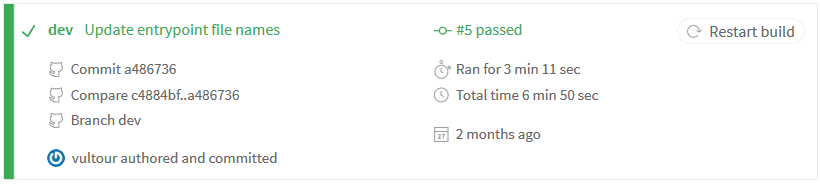
\includegraphics[width=\textwidth]{liebert-travis.png}
                \caption{An example result of a Travis CI build}
                \label{fig:travis}
            \end{figure}
        \end{center}
    \clearpage
    \section{Results}
    The application has been benchmarked using a simple strategy of inspecting its run-time process information on Linux. The data was gathered from a variety of sources, including raw Linux status files such as \textit{/proc/$<$pid$>$/status} or \textit{/proc/$<$pid$>$/sched}, or from system utilities such as \textit{htop}. In order to not only record the application's performance, but compare it to other established monitoring solutions, the same benchmark was also ran for two previously mentioned products - \textbf{Nagios} and \textbf{collectd} (\autoref{sec:similar-software}). These two competitors were chosen due to each of them being focused on a different aspect: features for \textit{Nagios}, and performance for \textit{collectd}.
    
    The benchmark consisted of a 30-minute session. After the time expired, a snapshot of the application state data was taken and inspected. The applications were ran with as closely matching configurations as possible (CPU \& memory metrics, 5 minute gather interval, localhost).
    
    
    \subsection{Nagios}
        Nagios fared surprisingly very well in the benchmark, especially CPU-wise. It's memory usage hovered around the \textbf{60 megabyte} mark. It utilized several single-threaded subprocesses, most notably several "worker" subprocess which appeared to be used for running the metric gathering and plugin architecture. The main process was the largest memory consumer with a stable \textbf{25MB}. 
        
        Inspecting the CPU consumption\footnote{CPU usage was determined using \textit{/proc/$<$pid$>$/sched}}, in total the main process used \textbf{1100ms}\footnote{Milliseconds, $1/1000$ of a second} of processor time. Out of this, \textbf{824ms} was consumed by the worker-handling subprocess.
        
        One very large disadvantage of Nagios is that it requires the \textit{apache} web server to function. Luckily, this is only required on the main Nagios server, not on all monitored nodes. It however massively increases the requirements for the server, as a bare-bones \textit{apache} install that was installed alongside Nagios consumed about \textit{400MB} of memory when running.
        
        \subsubsection{Limitations}
            There are several things that need to be noted for this benchmark. Firstly, the \textit{Nagios Core} version of the software has been used. This version sacrifices some features in favour of improved performance, therefore there may be a drastic difference between the two versions.
            
            Secondly, only the local machine metric gathering was tested. Nagios doesn't use the common server-client architecture, therefore it is very hard to determine its actual memory usage. In order to monitor remote nodes, one can either opt in to use a SSH based remote-execution module which is very inefficient with increasing number of nodes, or install \textit{NRPE} (Nagios Remote Plugin Executor) on remote nodes. The second option is preferred, however incurs a more severe performance penalty compared to SSH.
    
            
    \subsection{collectd}
        For the \textit{collectd} benchmark, 2 instances of the application were launched: one configured as a client metric gatherer, and another one as a server receiving data and storing it using the \textit{RRD} backend. 
        
        \subsubsection{Client}
            The client \textit{collectd} application consumed \textbf{18MB} of memory while running. After 30 minutes, its processor usage was \textbf{110ms}, most of which is attributed to the "worker" thread handling plugins.
            
        \subsubsection{Server}
            \textit{Collectd} in server configuration was using \textbf{16MB} of memory. \textbf{80ms} of processor time has been consumed during its execution, most of which is once again attributed to the plugin "worker" thread that handled an \textit{RRD} backend this time.
    
    
    \subsection{Liebert}
        \subsubsection{Agent}
            During the 30-minute benchmark run, our \textit{liebert-agent} application was consuming memory in the ballpark of \textbf{60MB}. During this time, it used \textbf{1380ms} of processor time. This time was evenly divided between the built-in CPU and memory gatherer threads. Inspecting the threads, we found out that they performed up to \textbf{60000 context switches}.
            
        \subsubsection{Controller}
            The controller application turned out to be surprisingly performant. Its memory usage was \textbf{50MB}, however processor time turned out to be only about \textbf{10 milliseconds} after 30 minutes. Half of the execution time came from the \textit{RRD} storage backend thread. Peculiarly, the network-related threads in both \textit{Agent} and \textit{Controller} only consumed about \textbf{1ms} each.
            
            
    \subsection{Discussion}
        \begin{figure}
            \centering
            \begin{tabular}{ |c|c|c| }
                \hline
                    Product & Memory usage & CPU time\\
                    \hline
                    \textbf{Nagios} & 60MB & 1100ms\\
                    \hline
                    \textbf{collectd (client)} & 18MB & 110ms\\
                    \hline
                    \textbf{collectd (server)} & 16MB & 80ms\\
                    \hline
                    \textbf{\textsc{Liebert} Agent} & 60MB & 1380ms\\
                    \hline
                    \textbf{\textsc{Liebert} Controller} & 50MB & 10ms\\
                \hline
            \end{tabular}
            \caption{Comparison table of benchmarked monitoring solutions}\label{fig:comparison-table-results}
        \end{figure}
        
        Looking at the test results in \autoref{fig:comparison-table-results}, it is clear that the project did not entirely fulfill its promise. Even though most of the code has been written with optimizations in mind, it didn't help us beat even the poorest performer in the benchmark, \textit{Nagios}.
        
        Looking deeper into the data, it is almost guaranteed that most of the inefficiencies of the \textit{Agent} application stem from its idling behaviour (described closer in \autoref{sec:notable-issues}). Looking at the context switching metric makes it clear that the idling behaviour is incredibly inefficient, and frequently requires scheduling on the CPU even when there is no work being done. Improving the waiting function to consume no CPU while idle would more than probably bump the application closer to the results of \textit{collectd}, possibly even close to the \textit{Controller}.
        
        The \textit{Controller} results are very surprising, given the amount of hidden inefficiencies discovered, such as the multi-threaded memory consumption or the inefficient wait function. This application however doesn't suffer from the wait function problem as all waiting is done through native blocking mechanisms, due to not having the requirements for which the incriminated function has been created. We could therefore venture as far as to say that this is the true image of \textsc{Liebert}, and given enough time it would be possible to get the \textit{Agent} application close to the \textit{Controller} resource usage.
        
        The resource usage of \textit{collectd} can most probably be attributed to its plugin system, as it needs to load and run the complex dispatch/receive routing architecture.
        
        Additionally it must be stated that even though our \textit{Controller} application beat the \textit{collectd} counterpart, it would be more fair to test in a large-scale environment with hundreds of clients, which is unfortunately impossible. This way \textit{collectd} could benefit from its years of optimizations, especially in the \textit{RRD} storage backend. It, for example, buffers multiple \textit{RRD} updates and executes them as a single command, compared to \textsc{Liebert} which executes them sequentially one-by-one. It is therefore almost given that in a large-scale test \textit{collectd} would outperform both \textit{Liebert} applications.
    \clearpage
    \section{Conclusions}
    \subsection{Discussion and Summary}
        In conclusion, the project fulfilled its primary objective to be a learning experience. Over the past few months it provided countless opportunities for expanding both theoretical and practical knowledge, be it in the form of learning the new programming language \textit{Rust}, or trying to figure out the intricacies of threads. During this time it also sparked numerous productive technical discussions with my peers, as well as online.
        
        Even though it is unfortunate that the goal of creating an efficient and fast monitoring solution has been unsuccessful, I believe that the groundwork has been laid. Should the development of the application continue, it is very possible that only a couple of changes could have tremendous effect on the overall efficiency of the application processor-wise. If the time to switch away from the multi-threaded model could be found (read more in the next section), it would very likely put the application on the forefront of efficiency in terms of memory.
        
        I can say in good faith that maximum effort has been put into optimizing the application wherever possible. In retrospect, this might not have been the best course of action, as a single large decision like the multi-threaded model managed to wipe out the endless stream of micro-optimizations undertaken during development. Even through all of this however, remnants of the optimizations still manage to shine through once in a while, such as was the case with performance of the \textit{Controller}. It is therefore pretty clear that most of the inefficiencies stem from inexperience and not willful ignorance of the requirements.


        \clearpage
    

\section{Possible Future Work and Enhancements}\label{sec:future-work}
    \subsection{Event model}
        A large portion of the application's inefficiencies (especially in memory consumption) comes from the threading model. Once these were discovered, an alternative model has been produced, unfortunately re-developing the application from the start was out of scope of the project. The new model uses a single main thread, and a configurable amount of \textit{worker} threads. The main thread acts as an event loop, continuously checking which plugins should be ran, and sending a message notifying one of the \textit{worker} threads to execute the plugin code once it's supposed to be scheduled. This would reduce the amount of required threads to a minimum of 4: main, worker, network reader, and network writer. There is no way of reducing the network thread requirement due to \textit{Rust}'s synchronous I/O.
        
        The synchronousness of \textit{Rust}'s I/O is unfortunately a bigger problem in the \textit{Controller} application, as it must spawn a new thread for each connected \textit{Agent}. This means that even though we could reduce the load imposed by unnecessary plugin thread spawning, we would still have potentially hundreds or thousands of threads being spawned for network communication purposes. Although their load might not be as significant, considering that their underlying code would be very similar, therefore they could utilize shared memory. It is still however an extreme overkill, be it from memory utilization, or the incredible amount of context switching required for such load. A more sensible solution would be to rewrite the \textit{Controller} application in a more network-friendly language. My personal favourite is Elixir\footnote{Basically an upgraded version of Erlang}, as it has something called \textit{processes}\footnote{Not to be confused with operating system processes}. \textit{Processes} are extremely lightweight (compared to OS processes or threads), isolated from one another, and run in parallel. A typical \textit{Elixir} application is able to handle thousands, or even tens of thousands, of processes with ease. This would unfortunately not fall in line with the project's vision, as it requires the installation of the Elixir / Erlang VM. \textsc{Liebert}, being written in \textit{Rust}, can be easily distributed in binary form and doesn't have any dependencies. Additionally, \textit{Rust} is built with cross-platform compatibility in mind, unlike many other languages (primary targets are Linux, Windows, and OSX).
        
    \subsection{Plugins}
        Regrettably, the plugin system has not been finished, therefore only core built-in gatherers and storage backends are currently available. Much of the infrastructure for plugin support has been put in place however, such as the custom format specifiers that can be reported and consumed by plugins. The actual plugin functionality is however not present in the current version of the project, as although it might look like a fairly simple task, it would probably require a lot of tinkering to get right. It has therefore been decided to leave this feature out in favour of other essential core features.
        
    \subsection{Code refactoring}
        As has previously been mentioned in multiple chapters, the code is currently nowhere near perfect. Often, tasks and problems were dealt with using semi-temporary workarounds or hacks due to time constraints. Furthermore, it would be very beneficial to split larger code blocks into separate functions to assist in testing. Refactoring the code to fix these issues would increase the overall quality and understandability, potentially allowing other people to collaborate on extending the project.
    \clearpage
    \section{Glossary}
    \begin{tabular}{ p{3.7cm}|p{11.5cm} }
        \textbf{Agent}          & Endpoint application of the platform (\autoref{sec:architecture})\\
        \textbf{CD}             & Continuous Delivery\\
        \textbf{CI}             & Continuous Integration\\
        \textbf{CLI}            & Command Line Interface\\
        \textbf{Controller}     & Central connection point of the platform (\autoref{sec:architecture})\\
        \textbf{CPU}            & Central Processing Unit (processor)\\
        \textbf{FFI}            & Foreign Function Interface\\
        \textbf{Heap}           & Thread-global dynamic memory region\\
        \textbf{I/O}            & Input / Output\\
        \textbf{IP (address)}   & Internet Protocol address\\
        \textbf{Jiffies}        & A processor utilization metric\\
        \textbf{kB}             & Kilobytes\\
        \textbf{MB}             & Megabytes\\
        \textbf{Metric}         & Measure of a system's property\\
        \textbf{Mutex}          & Object used for thread synchronization\\
        \textbf{RAII}           & Resource Acquisition Is Initialization pattern\\
        \textbf{Stack}          & Local function memory\\
        \textbf{TCP}            & Transmission Control Protocol\\
        \textbf{Thread panic}   & A manually induced crash in \textit{Rust}\\
        \textbf{TOML}           & Tom's Obvious, Minimal Language\\
    \end{tabular}
    \clearpage
    \section{References and Bibliography}
    \bibliographystyle{agsm}
    \bibliography{requirements}
    \clearpage
    \section{Appendices}
    
    \subsection{Appendix A: Network protocol specification}\label{apd:network}
        \begin{verbatim}
<data-spec> | <format-block>
                
data-spec:
    DATA <metric-name> <data1> [<data2> [...]]
                    
format-block:
    FORMAT <metric-name>
    <format-spec>
    [<format-spec>]
    [...]
    FORMAT END
                        
format-spec:
    <metric-type> <data-source> <heartbeat> <min> <max>
                        
metric-type: 1 | 2
<metric-type> represents RRD data source type:
    1 - gauge
    2 - counter
                        
metric-name, data-source: (a-zA-Z.-)
                    
heartbeat: unsigned 32-bit integer

min, max: U | signed 64-bit integer

data: signed 64-bit integer
        \end{verbatim}

    \subsection{Appendix B: Controller pmap output}\label{apd:pmap-controller}
        \begin{verbatim}
14103:   target/release/liebert-controller
Address           Kbytes     RSS   Dirty Mode  Mapping
000055e46320d000       0       0       0 r-x-- liebert-controller
000055e463568000       0       0       0 r---- liebert-controller
000055e463571000       0       0       0 rw--- liebert-controller
000055e463572000       0       0       0 rw---   [ anon ]
00007f6b13a00000       0       0       0 rw---   [ anon ]
00007f6b13ffe000       0       0       0 -----   [ anon ]
00007f6b13fff000       0       0       0 rw---   [ anon ]
00007f6b141ff000       0       0       0 -----   [ anon ]
00007f6b14200000       0       0       0 rw---   [ anon ]
00007f6b14bff000       0       0       0 -----   [ anon ]
00007f6b14c00000       0       0       0 rw---   [ anon ]
00007f6b151fd000       0       0       0 -----   [ anon ]
00007f6b151fe000       0       0       0 rw---   [ anon ]
00007f6b153fe000       0       0       0 -----   [ anon ]
00007f6b15600000       0       0       0 rw---   [ anon ]
00007f6b15cff000       0       0       0 r-x-- libm-2.21.so
00007f6b15e06000       0       0       0 ----- libm-2.21.so
00007f6b16005000       0       0       0 r---- libm-2.21.so
00007f6b16006000       0       0       0 rw--- libm-2.21.so
00007f6b16007000       0       0       0 r-x-- libc-2.21.so
00007f6b161be000       0       0       0 ----- libc-2.21.so
00007f6b163be000       0       0       0 r---- libc-2.21.so
00007f6b163c2000       0       0       0 rw--- libc-2.21.so
00007f6b163c4000       0       0       0 rw---   [ anon ]
00007f6b163c8000       0       0       0 r-x-- libgcc_s-5.3.1-20160406.so.1
00007f6b163de000       0       0       0 ----- libgcc_s-5.3.1-20160406.so.1
00007f6b165dd000       0       0       0 r---- libgcc_s-5.3.1-20160406.so.1
00007f6b165de000       0       0       0 rw--- libgcc_s-5.3.1-20160406.so.1
00007f6b165df000       0       0       0 r-x-- libpthread-2.21.so
00007f6b165f6000       0       0       0 ----- libpthread-2.21.so
00007f6b167f5000       0       0       0 r---- libpthread-2.21.so
00007f6b167f7000       0       0       0 rw--- libpthread-2.21.so
00007f6b167f8000       0       0       0 rw---   [ anon ]
00007f6b167fc000       0       0       0 r-x-- librt-2.21.so
00007f6b16803000       0       0       0 ----- librt-2.21.so
00007f6b16a02000       0       0       0 r---- librt-2.21.so
00007f6b16a03000       0       0       0 rw--- librt-2.21.so
00007f6b16a04000       0       0       0 r-x-- libdl-2.21.so
00007f6b16a07000       0       0       0 ----- libdl-2.21.so
00007f6b16c06000       0       0       0 r---- libdl-2.21.so
00007f6b16c07000       0       0       0 rw--- libdl-2.21.so
00007f6b16c08000       0       0       0 r-x-- ld-2.21.so
00007f6b16e01000       0       0       0 rw---   [ anon ]
00007f6b16e19000       0       0       0 rw---   [ anon ]
00007f6b16e28000       0       0       0 r---- ld-2.21.so
00007f6b16e29000       0       0       0 rw--- ld-2.21.so
00007f6b16e2a000       0       0       0 rw---   [ anon ]
00007ffe59340000       0       0       0 -----   [ anon ]
00007ffe59b1e000       0       0       0 rw---   [ stack ]
00007ffe59b88000       0       0       0 r----   [ anon ]
00007ffe59b8a000       0       0       0 r-x--   [ anon ]
ffffffffff600000       0       0       0 r-x--   [ anon ]
000055e463571000       4       4       4 rw--- liebert-controller
000055e463572000       4       4       4 rw---   [ anon ]
00007f6b13ffe000       4       0       0 -----   [ anon ]
00007f6b141ff000       4       0       0 -----   [ anon ]
00007f6b14bff000       4       0       0 -----   [ anon ]
00007f6b151fd000       4       0       0 -----   [ anon ]
00007f6b153fe000       4       0       0 -----   [ anon ]
00007f6b155ff000       4       0       0 -----   [ anon ]
00007f6b16005000       4       4       4 r---- libm-2.21.so
00007f6b16006000       4       4       4 rw--- libm-2.21.so
00007f6b165dd000       4       4       4 r---- libgcc_s-5.3.1-20160406.so.1
00007f6b165de000       4       4       4 rw--- libgcc_s-5.3.1-20160406.so.1
00007f6b167f7000       4       4       4 rw--- libpthread-2.21.so
00007f6b16a02000       4       4       4 r---- librt-2.21.so
00007f6b16a03000       4       4       4 rw--- librt-2.21.so
00007f6b16c06000       4       4       4 r---- libdl-2.21.so
00007f6b16c07000       4       4       4 rw--- libdl-2.21.so
00007f6b16e28000       4       4       4 r---- ld-2.21.so
00007f6b16e29000       4       4       4 rw--- ld-2.21.so
00007f6b16e2a000       4       4       4 rw---   [ anon ]
00007ffe59340000       4       0       0 -----   [ anon ]
ffffffffff600000       4       0       0 r-x--   [ anon ]
00007f6b163c2000       8       8       8 rw--- libc-2.21.so
00007f6b167f5000       8       8       8 r---- libpthread-2.21.so
00007ffe59b88000       8       0       0 r----   [ anon ]
00007ffe59b8a000       8       4       0 r-x--   [ anon ]
00007f6b16a04000      12      12       0 r-x-- libdl-2.21.so
00007f6b163be000      16      16      16 r---- libc-2.21.so
00007f6b163c4000      16      12      12 rw---   [ anon ]
00007f6b167f8000      16       4       4 rw---   [ anon ]
00007f6b16e01000      20      20      20 rw---   [ anon ]
00007f6b167fc000      28      16       0 r-x-- librt-2.21.so
000055e463568000      36      36      36 r---- liebert-controller
00007f6b16e19000      60       4       4 rw---   [ anon ]
00007f6b163c8000      88      88       0 r-x-- libgcc_s-5.3.1-20160406.so.1
00007f6b165df000      92      92       0 r-x-- libpthread-2.21.so
00007f6b16c08000     132     132       0 r-x-- ld-2.21.so
00007ffe59b1e000     136      48      48 rw---   [ stack ]
00007f6b15cff000    1052     192       0 r-x-- libm-2.21.so
000055e46320d000    1392    1228       0 r-x-- liebert-controller
00007f6b16007000    1756    1316       0 r-x-- libc-2.21.so
00007f6b15e06000    2044       0       0 ----- libm-2.21.so
00007f6b163de000    2044       0       0 ----- libgcc_s-5.3.1-20160406.so.1
00007f6b165f6000    2044       0       0 ----- libpthread-2.21.so
00007f6b16803000    2044       0       0 ----- librt-2.21.so
00007f6b16a07000    2044       0       0 ----- libdl-2.21.so
00007f6b13fff000    2048      12      12 rw---   [ anon ]
00007f6b151fe000    2048      12      12 rw---   [ anon ]
00007f6b153ff000    2048       8       8 rw---   [ anon ]
00007f6b161be000    2048       0       0 ----- libc-2.21.so
00007f6b13a00000    4096      48      48 rw---   [ anon ]
00007f6b14c00000    4096      24      24 rw---   [ anon ]
00007f6b15600000    6144     344     344 rw---   [ anon ]
00007f6b14200000    8192     116     116 rw---   [ anon ]
---------------- ------- ------- -------
total kB           45912    3856     776
        \end{verbatim}
            
    \pagebreak
            
    \subsection{Appendix C: Agent pmap output}\label{apd:pmap-agent}
        \begin{verbatim}
17380:   target/release/liebert-agent
Address           Kbytes     RSS   Dirty Mode  Mapping
000055dec76e1000       0       0       0 r-x-- liebert-agent
000055dec7aba000       0       0       0 r---- liebert-agent
000055dec7ac6000       0       0       0 rw--- liebert-agent
000055dec7ac7000       0       0       0 rw---   [ anon ]
00007fc7c3000000       0       0       0 rw---   [ anon ]
00007fc7c37fe000       0       0       0 -----   [ anon ]
00007fc7c37ff000       0       0       0 rw---   [ anon ]
00007fc7c39ff000       0       0       0 -----   [ anon ]
00007fc7c3a00000       0       0       0 rw---   [ anon ]
00007fc7c47fa000       0       0       0 -----   [ anon ]
00007fc7c47fb000       0       0       0 rw---   [ anon ]
00007fc7c49fb000       0       0       0 -----   [ anon ]
00007fc7c49fc000       0       0       0 rw---   [ anon ]
00007fc7c4bfc000       0       0       0 -----   [ anon ]
00007fc7c4bfd000       0       0       0 rw---   [ anon ]
00007fc7c4dfd000       0       0       0 -----   [ anon ]
00007fc7c4dfe000       0       0       0 rw---   [ anon ]
00007fc7c4ffe000       0       0       0 -----   [ anon ]
00007fc7c4fff000       0       0       0 rw---   [ anon ]
00007fc7c51ff000       0       0       0 -----   [ anon ]
00007fc7c5200000       0       0       0 rw---   [ anon ]
00007fc7c5829000       0       0       0 r-x-- libm-2.21.so
00007fc7c5930000       0       0       0 ----- libm-2.21.so
00007fc7c5b2f000       0       0       0 r---- libm-2.21.so
00007fc7c5b30000       0       0       0 rw--- libm-2.21.so
00007fc7c5b31000       0       0       0 r-x-- libc-2.21.so
00007fc7c5ce8000       0       0       0 ----- libc-2.21.so
00007fc7c5ee8000       0       0       0 r---- libc-2.21.so
00007fc7c5eec000       0       0       0 rw--- libc-2.21.so
00007fc7c5eee000       0       0       0 rw---   [ anon ]
00007fc7c5ef2000       0       0       0 r-x-- libgcc_s-5.3.1-20160406.so.1
00007fc7c5f08000       0       0       0 ----- libgcc_s-5.3.1-20160406.so.1
00007fc7c6107000       0       0       0 r---- libgcc_s-5.3.1-20160406.so.1
00007fc7c6108000       0       0       0 rw--- libgcc_s-5.3.1-20160406.so.1
00007fc7c6109000       0       0       0 r-x-- libpthread-2.21.so
00007fc7c6120000       0       0       0 ----- libpthread-2.21.so
00007fc7c631f000       0       0       0 r---- libpthread-2.21.so
00007fc7c6321000       0       0       0 rw--- libpthread-2.21.so
00007fc7c6322000       0       0       0 rw---   [ anon ]
00007fc7c6326000       0       0       0 r-x-- librt-2.21.so
00007fc7c632d000       0       0       0 ----- librt-2.21.so
00007fc7c652c000       0       0       0 r---- librt-2.21.so
00007fc7c652d000       0       0       0 rw--- librt-2.21.so
00007fc7c652e000       0       0       0 r-x-- libdl-2.21.so
00007fc7c6531000       0       0       0 ----- libdl-2.21.so
00007fc7c6730000       0       0       0 r---- libdl-2.21.so
00007fc7c6731000       0       0       0 rw--- libdl-2.21.so
00007fc7c6732000       0       0       0 r-x-- ld-2.21.so
00007fc7c692b000       0       0       0 rw---   [ anon ]
00007fc7c693f000       0       0       0 rw---   [ anon ]
00007fc7c6952000       0       0       0 r---- ld-2.21.so
00007fc7c6953000       0       0       0 rw--- ld-2.21.so
00007fc7c6954000       0       0       0 rw---   [ anon ]
00007ffdfc35d000       0       0       0 -----   [ anon ]
00007ffdfcb3b000       0       0       0 rw---   [ stack ]
00007ffdfcb6c000       0       0       0 r----   [ anon ]
00007ffdfcb6e000       0       0       0 r-x--   [ anon ]
ffffffffff600000       0       0       0 r-x--   [ anon ]
000055dec7ac6000       4       4       4 rw--- liebert-agent
000055dec7ac7000       4       4       4 rw---   [ anon ]
00007fc7c37fe000       4       0       0 -----   [ anon ]
00007fc7c39ff000       4       0       0 -----   [ anon ]
00007fc7c47fa000       4       0       0 -----   [ anon ]
00007fc7c49fb000       4       0       0 -----   [ anon ]
00007fc7c4bfc000       4       0       0 -----   [ anon ]
00007fc7c4dfd000       4       0       0 -----   [ anon ]
00007fc7c4ffe000       4       0       0 -----   [ anon ]
00007fc7c51ff000       4       0       0 -----   [ anon ]
00007fc7c5b2f000       4       4       4 r---- libm-2.21.so
00007fc7c5b30000       4       4       4 rw--- libm-2.21.so
00007fc7c6107000       4       4       4 r---- libgcc_s-5.3.1-20160406.so.1
00007fc7c6108000       4       4       4 rw--- libgcc_s-5.3.1-20160406.so.1
00007fc7c6321000       4       4       4 rw--- libpthread-2.21.so
00007fc7c652c000       4       4       4 r---- librt-2.21.so
00007fc7c652d000       4       4       4 rw--- librt-2.21.so
00007fc7c6730000       4       4       4 r---- libdl-2.21.so
00007fc7c6731000       4       4       4 rw--- libdl-2.21.so
00007fc7c6952000       4       4       4 r---- ld-2.21.so
00007fc7c6953000       4       4       4 rw--- ld-2.21.so
00007fc7c6954000       4       4       4 rw---   [ anon ]
00007ffdfc35d000       4       0       0 -----   [ anon ]
ffffffffff600000       4       0       0 r-x--   [ anon ]
00007fc7c5eec000       8       8       8 rw--- libc-2.21.so
00007fc7c631f000       8       8       8 r---- libpthread-2.21.so
00007ffdfcb6c000       8       0       0 r----   [ anon ]
00007ffdfcb6e000       8       4       0 r-x--   [ anon ]
00007fc7c652e000      12      12       0 r-x-- libdl-2.21.so
00007fc7c5ee8000      16      16      16 r---- libc-2.21.so
00007fc7c5eee000      16      12      12 rw---   [ anon ]
00007fc7c6322000      16       4       4 rw---   [ anon ]
00007fc7c692b000      20      20      20 rw---   [ anon ]
00007fc7c6326000      28      28       0 r-x-- librt-2.21.so
000055dec7aba000      48      48      48 r---- liebert-agent
00007fc7c693f000      76       4       4 rw---   [ anon ]
00007fc7c5ef2000      88      88       0 r-x-- libgcc_s-5.3.1-20160406.so.1
00007fc7c6109000      92      92       0 r-x-- libpthread-2.21.so
00007fc7c6732000     132     120       0 r-x-- ld-2.21.so
00007ffdfcb3b000     136      44      44 rw---   [ stack ]
00007fc7c5829000    1052     220       0 r-x-- libm-2.21.so
00007fc7c5b31000    1756    1276       0 r-x-- libc-2.21.so
000055dec76e1000    1896    1596       0 r-x-- liebert-agent
00007fc7c5930000    2044       0       0 ----- libm-2.21.so
00007fc7c5f08000    2044       0       0 ----- libgcc_s-5.3.1-20160406.so.1
00007fc7c6120000    2044       0       0 ----- libpthread-2.21.so
00007fc7c632d000    2044       0       0 ----- librt-2.21.so
00007fc7c6531000    2044       0       0 ----- libdl-2.21.so
00007fc7c37ff000    2048      44      44 rw---   [ anon ]
00007fc7c47fb000    2048      12      12 rw---   [ anon ]
00007fc7c49fc000    2048      12      12 rw---   [ anon ]
00007fc7c4bfd000    2048      12      12 rw---   [ anon ]
00007fc7c4dfe000    2048      16      16 rw---   [ anon ]
00007fc7c4fff000    2048       8       8 rw---   [ anon ]
00007fc7c5ce8000    2048       0       0 ----- libc-2.21.so
00007fc7c3000000    6144     892     892 rw---   [ anon ]
00007fc7c5200000    6144     428     428 rw---   [ anon ]
00007fc7c3a00000   12288     168     168 rw---   [ anon ]
---------------- ------- ------- -------
total kB           54644    5248    1812
            \end{verbatim}
            
    \begin{landscape}
        \subsection{Appendix D: Gantt chart}\label{apd:gantt}
                \vspace{1cm}
                \begin{ganttchart}[
                    vgrid,
                    hgrid,
                    x unit=1.32cm,
                    link/.style={-latex, draw=red, fill=red}
                ]{1}{16}
                    \gantttitle{September}{2}
                    \gantttitle{October}{2}
                    \gantttitle{November}{2}
                    \gantttitle{December}{2}
                    \gantttitle{January}{2}
                    \gantttitle{February}{2}
                    \gantttitle{March}{2}
                    \gantttitle{April}{2} \\
    
                    \ganttbar{Requirements}{1}{6}
                    \ganttbar[inline]{further requirement discovery}{8}{16} \\
                    \ganttbar{Architecture}{4}{8} \\
                    \ganttbar{Protocols}{4}{10} \\
                    \ganttbar{Rust basics}{1}{6} \\
                    \ganttbar{Initial version}{4}{9} \\
                    \ganttbar{Features}{10}{16}
                    \ganttbar[inline]{agile - scrum}{10}{16}\\
                    \ganttbar{Report}{3}{6}
                    \ganttbar[inline]{Requirements}{3}{6}
                    \ganttbar[inline]{Final report}{10}{16}
    
                    \ganttlink[link type=f-s]{elem5}{elem6}
                    \ganttlink{elem0}{elem1}
                    \ganttlink{elem9}{elem10}
                \end{ganttchart}
    \end{landscape}
    
    
    \subsection{Appendix E: Configuration structure}\label{apd:config}
        \begin{verbatim}
pub type ConfigurationMap   = HashMap<String, String>;
pub type ConfigurationMutex = sync::Arc<sync::Mutex<ConfigurationMap>>;

pub struct Configuration {
    conf: ConfigurationMutex
}

impl Configuration {
    pub fn new(c: ConfigurationMutex) -> Configuration {
        Configuration{ conf: c }
    }

    pub fn clone(&self) -> Configuration {
        Configuration{ conf: self.conf.clone() }
    }

    pub fn clone_inner(&self) -> ConfigurationMutex {
        self.conf.clone()
    }
}

impl Configuration {
    pub fn get(&self, path: &str) -> Option<String> {
        let c = self.conf.lock().expect("FATAL ERROR: Couldn't 
            lock configuration mutex");
        match c.get(path) {
            Some(item)  => { return Some((*item).clone()); }
            None        => { return None; }
        }
    }

    pub fn get_unsafe(&self, path: &str) -> String {
        self.get(path).expect(format!("FATAL ERROR: Couldn't find option '{}'
            in configuration", path).as_str())
    }
}

impl fmt::Debug for Configuration{
    fn fmt(&self, f: &mut fmt::Formatter) -> fmt::Result {
        let data = self.conf.lock().expect("FATAL ERROR: Couldn't 
            lock configuration mutex");
        data.fmt(f)
    }
}
        \end{verbatim}
        
    
    \pagebreak
    
    \subsection{Appendix F: An example integration test}\label{apd:integration-test}
        \begin{verbatim}
extern crate liebert;

use std::collections::HashMap;
use sync::{mpsc, Arc, Mutex};

#[test]
fn plugin_builtin_cpu() {
    let config = HashMap::new();
    config.insert("builtin.cpu.enabled",  "true");
    config.insert("builtin.cpu.interval", "1");

    let config = liebert::types::Configuration::new(
        Arc::new(Mutex::new(config))
    );
    let (tx, rx) = mpsc::channel();

    match liebert::agent::plugins
     ::builtin_cpu::start_builtin_cpu(config, tx) {
        Ok(meta) => {
            assert_eq!("builtin.cpu", meta.0);
        },
        Err(_) => { assert!(false); }
    }

    match rx.recv() {
        Ok(msg) => {
            match msg {
                liebert::agent::Message::Data(id, time, data) => {
                    assert_eq!("builtin.cpu", id);
                    assert(time > 0);

                    let mut iter = data.split_whitespace();
                    assert(i64::from_str(it.next()).is_ok());
                    assert(i64::from_str(it.next()).is_ok());
                    assert(i64::from_str(it.next()).is_ok());
                    assert(i64::from_str(it.next()).is_ok());
                    assert_eq!(None, it.next());
                },
                _ => { assert!(false); }
            }
        },
        Err(_) => { assert!(false); }
    }
}
        \end{verbatim}

\end{document}